\documentclass[11pt]{article}
\usepackage[utf8]{inputenc}
\usepackage[margin=1.25in]{geometry}
\usepackage{amsmath, amsfonts, amssymb}
\usepackage{subfig}
\usepackage[dvipsnames]{xcolor}
\definecolor{niceblue}{HTML}{236899}


\newcommand{\rev}[1]{{\color{niceblue} #1}}

\usepackage{hyperref}
\usepackage{nameref}
\hypersetup{
    colorlinks=true,
    linkcolor=black,
    filecolor=black,      
    urlcolor=niceblue,
    citecolor=niceblue,
    linkbordercolor = white
}
\usepackage{amsbsy}
\usepackage{epsfig}
\usepackage{subfig}
\usepackage{bm}
\usepackage{xspace}
\usepackage{color}
\usepackage{subfloat}
\usepackage{float}
\usepackage{lineno}
\usepackage{ragged2e}
\usepackage{placeins}
\usepackage{comment}
\usepackage{hanging} % for SI references... not necessary but looks nice

\makeatletter
\let\LN@align\align
\let\LN@endalign\endalign
\renewcommand{\align}{\linenomath\LN@align}
\renewcommand{\endalign}{\LN@endalign\endlinenomath}
\let\LN@gather\gather
\let\LN@endgather\endgather
\renewcommand{\gather}{\linenomath\LN@gather}
\renewcommand{\endgather}{\LN@endgather\endlinenomath}
\makeatother

\widowpenalty10000
\clubpenalty10000

\definecolor{darkgrey}{HTML}{A9A9A9}
\renewcommand\linenumberfont{\normalfont\bfseries\small\color{darkgrey}}
\modulolinenumbers[2]

\usepackage{booktabs}
\usepackage[round]{natbib}
\bibliographystyle{fishfish}
\bibpunct{(}{)}{,}{a}{}{,}
\usepackage{authblk}
\usepackage{pdflscape}

% Linux Libertine:
\usepackage{textcomp}
\usepackage[sb]{libertine}
\usepackage[varqu,varl]{inconsolata}% sans serif typewriter
\usepackage[libertine,bigdelims,vvarbb]{newtxmath} % bb from STIX
\usepackage[cal=boondoxo]{mathalfa} % mathcal
\useosf % osf for text, not math
\usepackage[supstfm=libertinesups,%
  supscaled=1.2,%
  raised=-.13em]{superiors}
\usepackage{setspace}

% for table formatting
\usepackage{array}
\newcolumntype{^}{>{\currentrowstyle}}

\newcommand{\PreserveBackslash}[1]{\let\temp=\\#1\let\\=\temp}
\newcolumntype{C}[1]{>{\PreserveBackslash\centering}p{#1}}
\newcolumntype{R}[1]{>{\PreserveBackslash\raggedleft}p{#1}}
\newcolumntype{L}[1]{>{\PreserveBackslash\raggedright}p{#1}}

\newcommand{\ml}[1]{{\color{red}#1}}
% \newcommand{\lar}[1]{{\color{purple}#1}}
% other colours: orange, magenta, sky blue, purple, grey

\newcommand*{\TitleFont}{%
      \usefont{\encodingdefault}{\rmdefault}{b}{n}%
      \fontsize{13}{15}%
      \selectfont}
      
\newcommand{\R}[1]{\label{#1}\linelabel{#1}}
% \newcommand{\lr}[1]{page~\pageref{#1}, line~\lineref{#1}}
\newcommand{\lr}[1]{line~\lineref{#1}}


\title{Multidimensional tracking of marine species redistribution under climate change}


\date{}

% Tentative order 
\author[1,*]{Federico Maioli} 
\author[1]{Daniël van Denderen}
\author[2]{Max Lindmark} 
\author[1]{Marcel Montany\`es} 
\author[3]{Eric J. Ward} 
\author[4]{Sean C. Anderson}
\author[1]{Martin Lindegren} 

\affil[1]{National Institute of Aquatic Resources, Technical University of Denmark, 2800 Kgs. Lyngby, Denmark}
\affil[2]{Department of Aquatic Resources, Institute of Marine Research, Swedish University of Agricultural Sciences, 453 30 Lysekil, Sweden}
\affil[3]{Conservation Biology Division, Northwest Fisheries Science Center, NOAA Fisheries, Seattle, WA 98112, USA}
\affil[4]{Pacific Biological Station, Fisheries and Oceans Canada, Nanaimo, BC V9T 6N7, Canada}


\begin{document}
\begin{spacing}{1.5}


\maketitle

\vspace*{\fill}
\noindent
Corresponding author: \href{mailto:fedma@aqua.dtu.dk}{fedma@aqua.dtu.dk}

\clearpage
\linenumbers
%\setcounter{secnumdepth}{0}
\setcounter{secnumdepth}{5}


\newpage

\section{Introduction}

The world’s oceans are warming rapidly, driving a major reorganization of marine biodiversity \citep{ipcc_ocean_2019}. As temperatures rise, many species respond by tracking their thermal niche ---the range of temperatures suitable for survival and reproduction \citep{grinnell_niche-relationships_1917}--- through shifts in geographic distribution \citep{lenoir_species_2020}. These shifts, typically towards higher latitudes or deeper waters, are among the most widespread biological responses to climate change \citep{parmesan_globally_2003, parmesan_ecological_2006, poloczanska_global_2013, poloczanska_responses_2016} and are reshaping ecosystems, challenging resource management, and redefining conservation priorities \citep{pinsky_preparing_2018, pecl_biodiversity_2017}. 

At the center of this transformation are continental shelfs. Continental shelfs sustain exceptional biodiversity and productivity, support some of the world’s largest fisheries, and contribute roughly X\% of the global marine catch \citep{watson_database_2017}. Shelf systems also experience warming at rates exceeding the global ocean average \citep[e.g.,][]{pershing_slow_2015, song_arctic_2023}, exposing resident species to accelerated thermal stress. Thus, continental shelves support high biodiversity and productivity while facing disproportionate exposure to climate-driven warming.

Climate change–driven range shifts in marine systems are well documented \citep{poloczanska_global_2013, burrows_geographical_2014}. Yet, most previous research has examined only a single spatial dimension—typically the poleward movement of range centroids \citep[e.g.][]{nye_changing_2009,  dulvy_climate_2008, pinsky_marine_2013}. This narrow focus oversimplifies species' responses to warming and may help explain why model predictions of range shifts both in terms of magnitude and direction often fail \citep{lawlor_mechanisms_2024, fredston_reimagining_2025}. Such limitations also hinder our ability to forecast future changes in species distribution and composition and design effective management and conservation measures. In reality, marine species rarely respond along a single axis. For instance, fish may track their thermal niche by shifting in space, moving into deeper waters, and/or remain in place and experience increased thermal exposure \citep{nye_changing_2009}. Considering shifts in multiple directions and their potential interactions offers a more realistic representation of climate-driven redistribution of marine fishes.

To that end, we here develop and apply a multidimensional framework that considers three complementary dimensions of climate response: (i) horizontal range shifts, captured through changes in range centroids; (ii) vertical redistributions, reflected in realized depth niches; and (iii) changes in realized thermal niches, which reveal whether species are increasingly exposed to warming. While even broader approaches have been advocated \citep{fredston_reimagining_2025}, our focus on spatial and thermal axes captures the primary pathways by which marine fish interact with rapid ocean warming.

Our study draws on a comprehensive set of standardized scientific bottom-trawl surveys, including more than 200 well sampled demersal (bottom-living) fish populations across 11 regions of the North Atlantic and Northeast Pacific. These regions include some of the fastest-warming continental shelf seas, span broad latitudinal and climatic gradients, and provide some of the world's most comprehensive long-term records of marine biodiversity change \citep{maureaud_are_2021, maureaud_fishglob_data_2024}. Using a combination of spatiotemporal generalized linear mixed-effects models and Bayesian mixed-effects models, we quantify long-term trends in marine fish species range centroids, depth niches, and thermal niches, evaluate whether consistent patterns emerge across regions, and assess whether distinct combinations of responses correspond to coherent strategies. Finally, we test whether these strategies are associated with changes in population abundance, potentially distinguishing species that are adapting to warming conditions from those in decline.

%By integrating these metrics, we can disentangle true movements from passive thermal exposure and uncover how different response pathways interact.

\section{Methods}

\subsection{Data sources}

\subsubsection{Fish data}

Fish density data (kg/km\textsuperscript{2}) were obtained from 
a large-scale compilation of standardized, fishery-independent bottom-trawl surveys \citep{maureaud_fishglob_data_2024}. Each trawl deployment (haul) records the catch by species, with biomass standardized by the sampled ("swept") area, alongside the haul’s location, depth, and time. We selected surveys with a consistent sampling protocol and temporal coverage of at least 15 years \citep{maureaud_fishglob_data_2024}, resulting in 17 surveys across 11 regions (Fig \ref{fig:map}).

\begin{figure}[h]
    \centering
    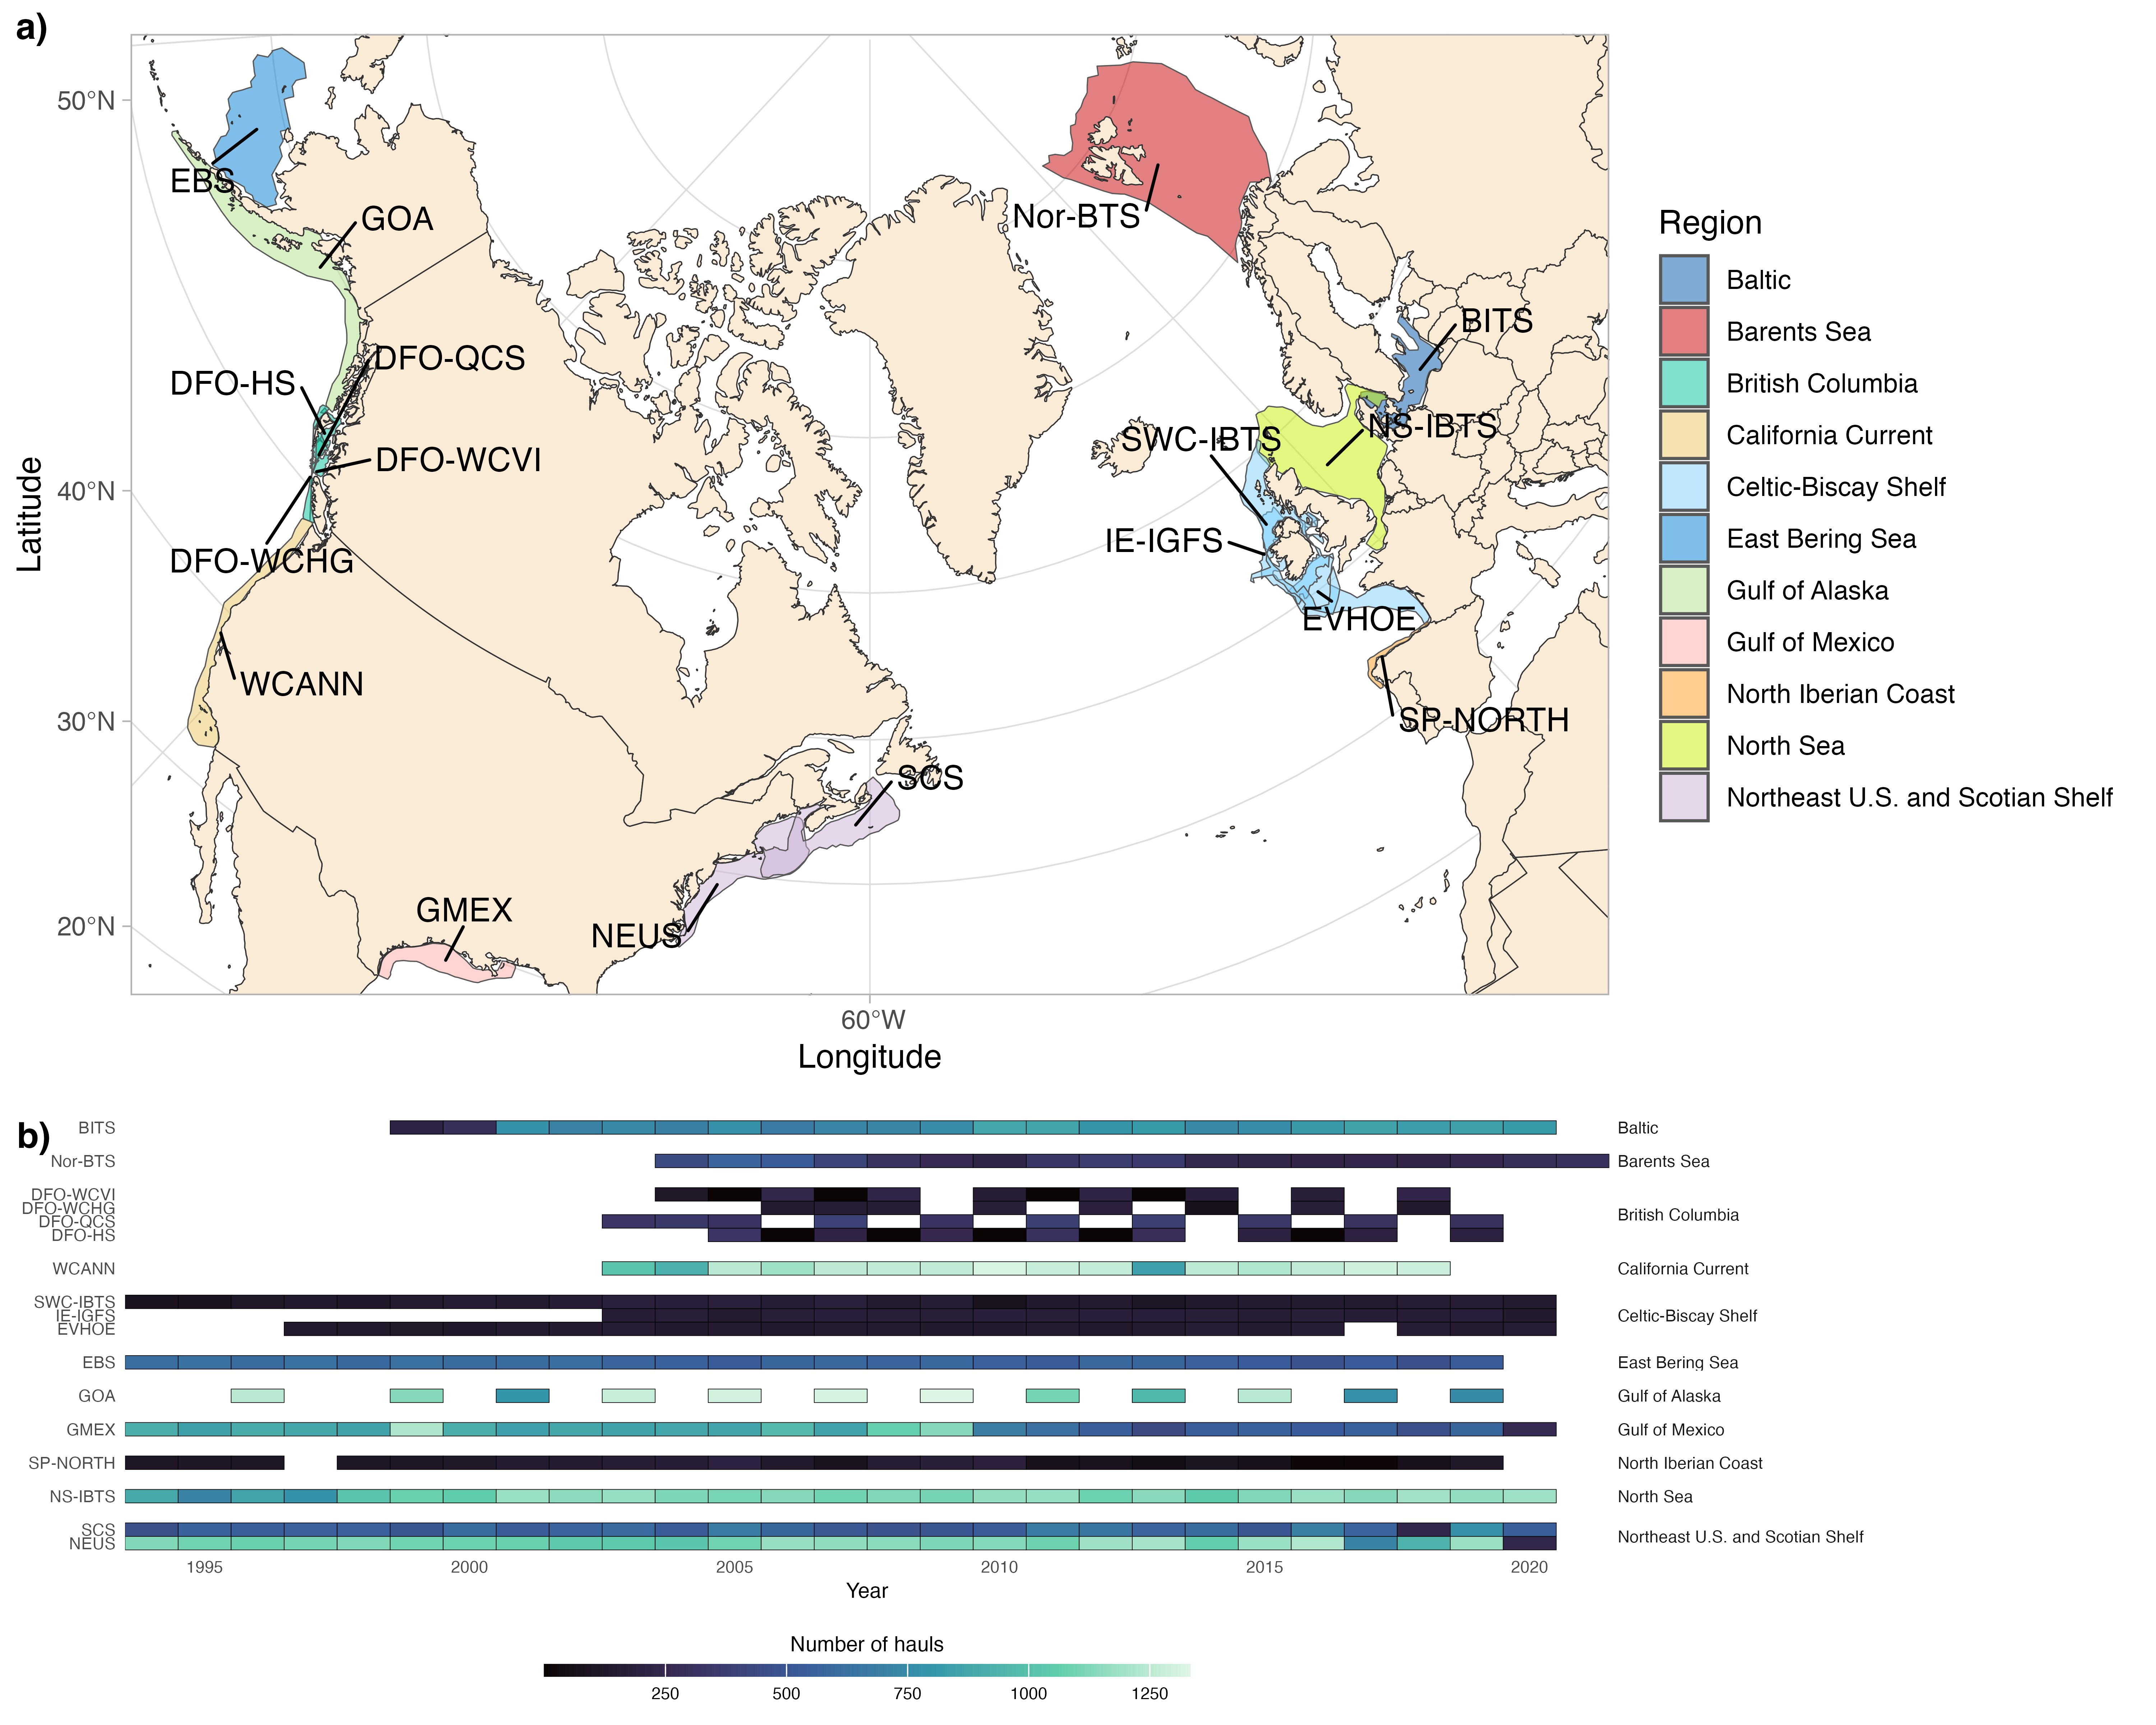
\includegraphics[scale=0.7]{output/figures/map.png}
\caption{Overview of survey data. (a) Map showing the surveys and ecoregions considered in the analysis. (b) Number of hauls per survey by year.}
    \label{fig:map}
\end{figure}

To avoid sampling bias and ensure robust estimation of the spatial and temporal dynamics of species, we retained only taxa that (i) contributed 99\% of the cumulative biomass within each region and (ii) occurred in at least 15\% of hauls within that region. This filtering yielded a final dataset of 237 fish populations (species–region combinations) across all regions (Table S).


\subsubsection{Temperature data}

Since most observations lack in situ measurements of bottom temperature, we used monthly bottom temperature data derived from the Copernicus Global Ocean Physics Reanalysis \citep{european_union-copernicus_marine_service_global_2018}, which provides values on a regular grid with a spatial resolution of 1/12$^{\circ}$ (approximately 7 km at the study latitudes).

%Where possible, we validated the model-derived temperatures against available in situ measurements, finding good agreement between the two (Appendix Fig. SX).

\subsection{Species spatiotemporal modeling}\label{sec:Species spatiotemporal modeling}

To model species distributions and how they have changed over time, we employed spatiotemporal generalized linear mixed-effects models (GLMMs), a flexible and widely used approach in fisheries science \citep{thorson_geostatistical_2015, thorson_model-based_2016}. For each species analyzed (S1 Table), we modeled biomass density as a Tweedie-distributed response, appropriate for data containing a combination of zeroes and continuous positive values. 
The general form of the spatiotemporal GLMM can be represented as:
\begin{align}
    y_{s,t} &\sim \text{Tweedie} \left( \mu_{\boldsymbol{s},t}, p, \phi \right), \quad 1 < p < 2, \label{eq:1} \\
    \mu_{s,t} &= \exp \left( X_{\boldsymbol{s},t} \beta + \omega_{\boldsymbol{s}} + \epsilon_{\boldsymbol{s},t} \right), \label{eq:2} \\
    \omega &\sim \operatorname{MVN} \left(0, \Sigma_{\omega} \right), \label{eq:3} \\
    \epsilon_{t} &\sim \operatorname{MVN} \left(0, \Sigma_{\epsilon} \right), \label{eq:4}
\end{align}
where \( y_{\mathbf{s},t} \) represents fish density (kg/km\(^2\)) at spatial location \( \mathbf{s} \) and time \( t \), \( \mu \) is the expected mean CPUE, and \( p \) and \( \phi \) are the power and dispersion parameters of the Tweedie distribution, respectively. \( \mathbf{X}_{\mathbf{s},t} \) is the design matrix of covariates including year (as a categorical variable) and a second-degree polynomial of log(depth), consisting of both linear and quadratic terms. The vector \( \bm{\beta} \) contains the corresponding fixed-effect coefficients.
We included log-transformed depth as a second-order polynomial to help constrain predictions to plausible magnitudes across the depth gradient.

Because fish species are not constrained by survey boundaries, and some surveys cover only a small part of the distribution range of species we aggregated multiple surveys into broader regions for modeling when appropriate. Surveys with extensive and clearly defined coverage (e.g., the North Sea IBTS) were modeled independently, while those with contiguous spatial domains and partial overlap in time and space (e.g., surveys conducted in British Columbia) were combined (Fig \ref{fig:map}). When multiple surveys were present within a region, we included survey identity as a fixed effect to account for potential differences in sampling. To capture intra-annual variability, we also included a month-specific random intercept for surveys spanning more than three months: $\alpha_m \sim \mathcal{N}(0, \sigma_{\alpha_m}^{2})$, where \textit{m} indexes the sampled months.

The parameters \( \omega_{\mathbf{s}} \) and \( \epsilon_{\mathbf{s},t} \) (Equations \ref{eq:3}--\ref{eq:4}) represent spatial and spatiotemporal random effects, respectively, both modeled as Gaussian Markov random fields \citep{lindgren_explicit_2011}. The spatial random field is shared across years, and represents static spatial effects such as habitat that are not accounted for by the fixed effects, while the spatiotemporal fields represent interannual spatial variation. We assumed spatiotemporal random fields to be independent across years to capture annual variation in spatial structure. While a first-order autoregressive (AR1) process could have been used to model temporal dependence, we opted for the independent formulation to strike a balance between computational efficiency and model flexibility. This approach allows spatial patterns to vary freely from year to year, accommodating potential non-stationary dynamics in species distributions without imposing strict temporal correlation structures.

For British Columbia surveys, which have a biennial sampling structure, we modeled spatiotemporal variation as a random walk process. This modifies Equation \ref{eq:4} into $\epsilon_{\boldsymbol{s},t} \sim  \operatorname{MVN}(\epsilon_{t-1},\Sigma_{\epsilon})$ to allow for flexibility in estimating the spatial and temporal processes in years without data \citep{ward_win_2024}.

Latent spatial and spatiotemporal random fields were approximated using a triangulated mesh with a minimum spacing (cutoff) of 20 km constructed with the \texttt{fmesher} R package \citep{lindgren_fmesher_2025}. This cutoff distance represents the smallest allowed distance between two mesh vertices. We assumed a shared range parameter between the spatial and spatiotemporal fields, while allowing each field to have its own variance.

The maximum marginal log-likelihood was estimated using Template Model Builder \citep[TMB;][]{kristensen_tmb_2016}, which applies the Laplace approximation to integrate out random effects. Models were fit in R 4.1.0 \citep{r_core_team_r_2021} using the \texttt{sdmTMB} package \citep{anderson_sdmtmb_2024}, which interfaces TMB with INLA-based spatial methods \citep{rue_approximate_2009}. Only models with a positive-definite Hessian and a maximum absolute log-likelihood gradient $< 0.001$ were considered successfully converged and used for inference \citep{anderson_sdmtmb_2024}.



\subsubsection{Prediction grid}

After model fitting and validation We predicted species-specific densities on a 4 $\times$ 4 km spatial grid (in local UTM coordinates) covering each region for all years with available data. Bathymetric information was extracted at the centroid of each grid cell from GEBCO \citep{gebco_bathymetric_compilation_group_2023_gebco_2023_2023}, which provides a bathymetric grid with a horizontal resolution of 0.00417° (approximately 400 m at our study latitudes).
Similarly, at each grid cell centroid, we extracted the average monthly temperature for the 12 months preceding the earliest survey month from the Copernicus Global Ocean Physics Reanalysis dataset.

\subsubsection{Spatial and thermal metrics}\label{sec:Spatial and thermal metrics}

To assess how species respond to ocean warming, we calculated annual metrics that capture both spatial redistribution and thermal exposure, namely range centroids (latitude and longitude), realized depth niche, and realized thermal niche. 
We estimated horizontal shifts in distribution using range centroids rather than range edges, since centroids have shown to be less prone to noise and provide a clearer signal of range-wide movement, thereby offering more stable and representative measures of geographic displacement \citep{shoo_detecting_2006}.
The centroids were estimated as the biomass-weighted mean latitude and longitude (center of gravity) across grid cells. Realized depth and thermal niches were computed as biomass-weighted averages of depth and temperature, respectively, representing the environmental conditions most heavily occupied by each species (Table~\ref{table:derived_quantities}). All metrics were derived from biomass densities predicted on the prediction grid using the fitted the spatiotemporal models. 

\begin{table}[h!]
\caption{Summary of derived spatial and thermal metrics. All statistics are calculated using predicted species density across grid cells.}
\centering
\renewcommand{\arraystretch}{1.5}
\begin{tabular}{
    >{\raggedright\arraybackslash}p{3.2cm} 
    >{\raggedright\arraybackslash}p{3.5cm} 
    >{\raggedright\arraybackslash}p{5cm} 
    >{\raggedright\arraybackslash}p{4.3cm}
}
\toprule
\textbf{Name} & \textbf{Metric} & \textbf{Definition / Formula} & \textbf{Interpretation} \\
\midrule

\textbf{Range centroid (latitude)} & Density-weighted latitude & 
$\bar{y} = \frac{\sum y_i D_i}{\sum D_i}$, where $y_i$ is the UTM northing of grid cell $i$, and $D_i$ is predicted density. & 
Tracks north–south distributional shifts. \\

\textbf{Range centroid (longitude)} & Density-weighted longitude & 
$\bar{x} = \frac{\sum x_i D_i}{\sum D_i}$, where $x_i$ is the UTM easting of grid cell $i$. & 
Tracks east–west distributional shifts. \\

\textbf{Depth niche} & Density-weighted depth & 
$\bar{z} = \frac{\sum z_i D_i}{\sum D_i}$, where $z_i$ is depth in grid cell $i$. & 
Captures changes in vertical habitat use. \\

\textbf{Thermal niche} & Density-weighted temperature & 
$\bar{T} = \frac{\sum T_i D_i}{\sum D_i}$, where $T_i$ is bottom temperature in grid cell $i$. & 
Reflects thermal conditions in occupied habitat. \\

\bottomrule
\end{tabular}
\label{table:derived_quantities}
\end{table}

\subsubsection{Population abundance}

For estimating abundance of each fish population, we calculated an area-weighted relative population abundance index by multiplying biomass density by cell area, summing these relative biomass values, and applying a generic bias correction \citep{thorson_geostatistical_2015, thorsonImplementingGeneric2016}. We then estimated population-specific temporal trends in abundance by fitting a linear model to the log-transformed annual indices.

\subsection{Bayesian trend analysis}\label{sec:Bayesian trend analysis}

We estimated trends in the set of spatial and thermal metrics discribed above using multivariate Bayesian mixed-effects models because these metrics are often correlated. For example, depth shifts can co-occur with changes in range centroid, and we modeled them jointly to capture shared variation. We initially modelled the outcomes using a multivariate normal (MVN) distribution, but posterior predictive checks revealed heavier tails than the MVN could capture, so we refitted the model using univariate Student-t distribution for each response, which are more robust to extreme values \citep[e.g.,][]{anderson_black-swan_2017}. Residual correlations across responses were retained using a multivariate normal correlation structure. This change improved predictive accuracy, as confirmed by higher leave-one-out cross-validation (LOO) scores \citep{vehtari_practical_2017} (Supplementary Table~\ref{tab:elpd}).

Next, we compared two alternative random-effects structures using LOO cross-validation: (i) random slopes varying by species–region combinations, and (ii) a hierarchicalstructure with species nested within regions. The nested specification was better supported and was therefore adopted for all subsequent analyses (Supplementary Table~\ref{tab:elpd}). This hierarchical framework improved model fit and, importantly, allowed us to estimate global, regional, and species-level trends within a single unified model.

An alternative would have been to fit separate models for each species and outcome. But this ignores information shared across taxa, regions, and outcomes. Instead, a hierarchical specification applies partial pooling: estimates draw strength from the broader dataset while still allowing region- and species-specific deviations. This shrinkage produces estimates that are more stable than those from independent fits (Supplementary Fig.~\ref{fig:shrinkage}; \citealt{mcelreath_statistical_2018}).


To improve interpretability and aid in model convergence, we normalized both the response variables and the time predictor within each species–region combination so that their mean is zero. As a result, the intercept can be omitted. We then rescaled time to decades, so that the slope can be interpreted directly as the rate of change per decade.
Thus the model can be written as:

\begin{align}
y_{i}^{(j)} &\sim \operatorname{Student-t}\left(\nu^{(j)}, \mu_{i}^{(j)}, \sigma^{(j)}\right),\qquad j=1,\dots,4,\\
\mu_{i}^{(j)} &= \beta^{(j)} \cdot \text{decade}_{i} + \beta_{\text{region}[r[i]]}^{(j)} \cdot \text{decade}_{i} + \beta_{\text{species}[s[i]]}^{(j)} \cdot \text{decade}_{i},\label{eq:linearpred} \\
\boldsymbol{\Sigma} &=
\begin{bmatrix}
\sigma_1^2 & \rho_{12}\sigma_1\sigma_2 & \rho_{13}\sigma_1\sigma_3 & \rho_{14}\sigma_1\sigma_4 \\
\rho_{21}\sigma_2\sigma_1 & \sigma_2^2 & \rho_{23}\sigma_2\sigma_3 & \rho_{24}\sigma_2\sigma_4 \\
\rho_{31}\sigma_3\sigma_1 & \rho_{32}\sigma_3\sigma_2 & \sigma_3^2 & \rho_{34}\sigma_3\sigma_4 \\
\rho_{41}\sigma_4\sigma_1 & \rho_{42}\sigma_4\sigma_2 & \rho_{43}\sigma_4\sigma_3 & \sigma_4^2
\end{bmatrix},\\
% OR
\begin{bmatrix}
\varepsilon_i^{(1)} \\ \varepsilon_i^{(2)} \\ \varepsilon_i^{(3)} \\ \varepsilon_i^{(4)}
\end{bmatrix}
&\sim \operatorname{MVN}\!\left(
\mathbf{0},\ 
\operatorname{diag}(\sigma_1,\sigma_2,\sigma_3,\sigma_4)\;
\mathbf{R}\;
\operatorname{diag}(\sigma_1,\sigma_2,\sigma_3,\sigma_4)
\right).
\end{align}

\vspace{1em}

\noindent Here, $y^{(j)}_i$ denotes the response variable $j$ for observation $i$, where $j$ is the latitudinal centroid,
longitudinal centroid, depth niche or thermal niche (Table \ref{table:derived_quantities}). The linear predictor (Eq \ref{eq:linearpred}) includes a global slope of decade for response $j$, denoted $\beta^{(j)}$, along with a deviation in slope for region $r$, $\beta^{(j)}_{\text{region}[r[i]]}$, and a deviation in slope for species $s$ within region, $\beta^{(j)}_{\text{species}[s[i]]}$. Finally,
$\boldsymbol{\Sigma}$ represents the residual covariance matrix capturing residual correlations among the response variables. The scale parameters $\sigma^{(j)}$ are estimated as part of the Student-t and the residual correlation matrix $\mathbf{R}$ controls how residuals co-vary across responses.

We used weakly informative priors for the global slopes (decade effects), guided by published rates of range shifts, depth changes, and ocean warming. For latitudinal and longitudinal centroids, we specified Normal$(0, 50)$ km decade$^{-1}$ priors, which accommodate range shifts up to ~30 km decade$^{-1}$ observed in marine taxa \citep{poloczanska_global_2013}. For depth, we used a Normal$(0, 5)$ m decade$^{-1}$ prior, consistent with estimates of ~3.6 m decade$^{-1}$ deepening in North Sea demersal fish \citep{dulvy_climate_2008}. For thermal niches, we applied a Normal$(0, 0.5)$ °C decade$^{-1}$ prior, encompassing values comparable to the ~0.37 $^\circ$C decade$^{-1}$ observed in rapidly warming shelf seas \citep{chen_longterm_2020}.
For group-level variation in slopes (the standard deviation of year effects), we used $\operatorname{Student-t}$ distributions truncated to $(0,\infty)$ with 3 degrees of freedom, allowing a wide range of biologically plausible variation. Priors were $\operatorname{Student-t}(3, 0, 30)$ km decade$^{-1}$ for spatial centroids, $\operatorname{Student-t}(3, 0, 10)$ m decade$^{-1}$ for depth, and $\operatorname{Student-t}(3, 0, 0.2)$ $^\circ$C decade$^{-1}$ for thermal niches. For species nested within regions, we specified slightly broader priors: $\operatorname{Student-t}(3, 0, 40)$ km decade$^{-1}$ for spatial centroids, $\operatorname{Student-t}(3, 0, 20)$ m decade$^{-1}$ for depth, and $\operatorname{Student-t}(3, 0, 0.4)$ $^\circ$C decade$^{-1}$ for thermal niches. These priors were validated against empirical distributions from the data to ensure consistency with observed variability (Supplementary Fig.~\ref{fig:priors}).

We fit models in R using the \texttt{brms} package \citep{burkner_brms_2017}, which interfaces with Stan via \texttt{rstan} \citep{stan2024,stan_development_team_rstan_2024}. All other priors followed \texttt{brms} defaults. Each model ran with four Markov chain Monte Carlo (MCMC) chains of 4,000 iterations, discarding the first 2,000 as warm-up. The remaining 2,000 samples per chain (8,000 total post–warm-up draws) formed the posterior distribution. Convergence was confirmed by $\hat{R} < 1.01$, absence of divergent transitions, and effective sample sizes $>$ 400 for all key parameters \citep{vehtari_rank-normalization_2021}.


\subsection{Expected shifts from thermal envelopes and climate analogs mapping}

To estimate expected shifts based on thermal changes, we applied two common methods for calculating spatially explicit climate velocities: thermal envelope shifts \citep{pinsky_marine_2013} and climate analog mapping \citep{fitzpatrick_contemporary_2019}. Thermal envelope shifts measure climate change velocity as the movement of isotherms across thermal gradients. This provides a directional estimate of how rapidly and in which direction species' thermal niches are expected to shift. In contrast, climate analog mapping identifies the regions where future climatic conditions resemble those of a reference location during a baseline period. This statistical approach maps areas of climatic similarity over time rather than assuming continuous displacement along gradients. Finally, we compared expected and observed shifts by testing both the strength of their correlation and their directional alignment.

\subsubsection{Thermal envelopes}

To estimate population-specific shifts expected under climate-driven thermal change, we fit simplified species distribution models using only temperature predictors. These models followed the structure in \textit{\nameref{sec:Species spatiotemporal modeling}}), but excluded spatial and spatiotemporal random fields to isolate temperature effects.

We modeled predicted density as a function of year and two temperature-based smooth terms:
\begin{equation}
\text{Density} \sim \beta_t + f_1(\text{MeanTemp}) + f_2(\text{MaxTemp})
\label{eq:8}
\end{equation}
Here, $\beta_t$ is a year-specific intercept (treated as a factor), and $f_1$ and $f_2$ are smooth functions estimated with penalized splines using $k = 3$ basis functions. MeanTemp is the average bottom temperature over the 12 months preceding the earliest survey month; MaxTemp is the temperature of the warmest month in that period. The spline terms allow for nonlinear species–temperature relationships. Models were fit using the \texttt{sdmTMB} R package.

We then derived spatial metrics (range centroid and depth niche) from the fitted values and assessed their temporal trends using the Bayesian framework described in \textit{\nameref{sec:Bayesian trend analysis}}). These temperature-only models provide climate envelope-based expectations under thermal forcing.

\subsubsection{Climate analogs}

To estimate expected shifts based on climate analogs, we conducted a spatial grid search for climate analogs at 4 km resolution across each region. For every grid cell, we identified locations in the final five years of the survey period that were climatically analogous to the estimated thermal niche in the first five years. Thermal niches were calculated (as in \textit{\nameref{sec:Spatial and thermal metrics}}) separately for minimum, maximum, and mean bottom temperatures over the 12 months preceding the earliest survey month.

For each temperature metric, we applied a non-parametric Wilcoxon rank-sum test to compare the distribution of thermal niche values between the baseline (first five years) and final period. Grid cells where the null hypothesis of equal distributions was not rejected ($p \geq 0.05$) were considered climate analogs, while those with $p < 0.05$ were classified as novel climates.

To define analog zones, we retained grid cells identified as analogs for each temperature variable (minimum, maximum, and mean) individually and overlaid the results. We then estimated the direction and magnitude of climate displacement by calculating the geographic distance between the range centroid of the first survey year and the nearest analogs (within the 10\textsuperscript{th} percentile of all distances) in the final five years. The median shift in both the longitudinal and latitudinal axes represented the expected displacement under thermal climate analogs.


\newpage

\section{Results}

\subsection{No net spatial shifts, but widespread niche warming across species and regions}

Overall, we found no consistent directional shifts across species and regions in either latitude or longitude over time, as indicated by 95\% Credible Intervals (CIs) overlapping zero. In our Bayesian regression model, the posterior mean global slope ($\beta_{\text{decade}}$) for latitudinal shift was 0.35 km decade$^{-1}$ [95\% CI: -8.04, 8.82], and for longitudinal shift was -2.73 km decade$^{-1}$ [95\% CI: -8.82, 2.88] (Fig. \ref{fig:effsize}). In contrast, we observed modest support for cross-regional trends in species deepening and strong support for thermal niche warming. The global slope for depth shift was 0.6 m decade$^{-1}$ [95\% CI: -0.53, 1.64], whereas for thermal niche shift it was 0.18 $^{\circ}$C decade$^{-1}$ [95\% CI: 0.07, 0.29] (Fig. \ref{fig:effsize}a).


\subsection{Regional variation in species shifts}

Region-wide community trends revealed that horizontal shifts were generally weak and inconsistent, whereas vertical and thermal niche shifts were more frequent and pronounced (Fig. \ref{fig:effsize}b). 

Latitudinal shifts varied among regions, with the highest proportion of species demonstrating significant changes (i.e., 95\% CIs excluding zero) in the North Sea (NS; 73\%) and Celtic-Biscay Shelf (CBS; 64\%), and fewer in the Gulf of Mexico (GMX; 15\%) and Gulf of Alaska (GOA; 14\%) and none in the Northern Iberian Coast (NIC; Supplementary Fig. \ref{fig:prop_sign}). Interestingly, both northward and southward responses were roughly balanced across most regions, although NS showed more northward movements (53\%) and the Baltic Sea (BAL) more southward (63\%). The only region with a clearly significant mean latitudinal shift was British Columbia (BC), showing a southward change of $-16.74$ km decade$^{-1}$ [95\% CI: $-30.44$, $-2.93$].

Longitudinal shifts  were generally weaker, with the highest proportion of species showing significant changes found in NS (80\%) and GMX (51\%), while only few species were found in CBS (10\%) and in the California–Oregon–Washington region (COW; 3\%). Eastward and westward movements were both observed, with NS showing predominantly westward shifts (53\%).

Depth-related shifts were most pronounced in BC (66\%) and NS (60\%), with species mainly moving to deeper waters in the northeast U.S. and Scotian Shelf (NEUS; 52\%) and BC (45\%) (Supplementary Fig. \ref{fig:prop_sign}). Significant shifts towards greater depths were found in BC ($1.97$ m decade$^{-1}$ [95\% CI: $0.40$, $3.80$]) and NEUS ($1.84$ m decade$^{-1}$ [95\% CI: $0.32$, $3.50$]), while BAL and Barents Sea (BS) showed lower proportions of significant changes in depth distribution (0–31\%).

In contrast to the spatial shifts above, thermal niche shifts were widespread and consistent across most regions (Supplementary Fig. \ref{fig:prop_sign}. More specifically, nearly all species in BC, CBS, COW, GMX, GOA, NEUS, and NS exhibited significant warming responses, with rates ranging from $0.13^{\circ}$C decade$^{-1}$ (CBS, COW) to $0.53^{\circ}$C decade$^{-1}$ in NEUS. Only NIC, EBS , and BS lacked significant thermal shifts.


\subsection{Species-specific responses}

Of the 237 fish populations assessed, approximately 38\% showed significant latitudinal shifts (Fig.~\ref{fig:effsize}c), with 48 species moving northward (20\%) and 43 southward (18\%). The most extreme northward shift was observed in \textit{Trisopterus minutus} in the NS ( 120.10 km decade$^{-1}$), and the strongest southward shift in \textit{Scyliorhinus canicula} in NS (-95.52 km decade$^{-1}$).  
Longitudinal shifts were significant for 35\% of species, with 50 shifting westward (21\%) and 32 shifting eastward. The largest eastward shift occurred in \textit{Harengula jaguana} in the GMX (107.39 km decade$^{-1}$), and the greatest westward shift in \textit{Merluccius bilinearis} in the NEUS (-68.49 km decade$^{-1}$).  
Depth shifts were significant for 34\% of species, with 48 species moving deeper (20\%) and 33 shallower. The strongest deepening occurred in \textit{Sebastes reedi} in BC (-13.04 m decade$^{-1}$), and the greatest shallowing in \textit{Squalus suckleyi} in BC (22.94 m decade$^{-1}$).  
Thermal niche shifts were the most widespread, with 78\% of species showing significant warming responses and none cooling. The largest positive response was in \textit{Urophycis tenuis} in NEUS (0.56 $^\circ$C decade$^{-1}$).  


\begin{figure}[h]
    \centering
    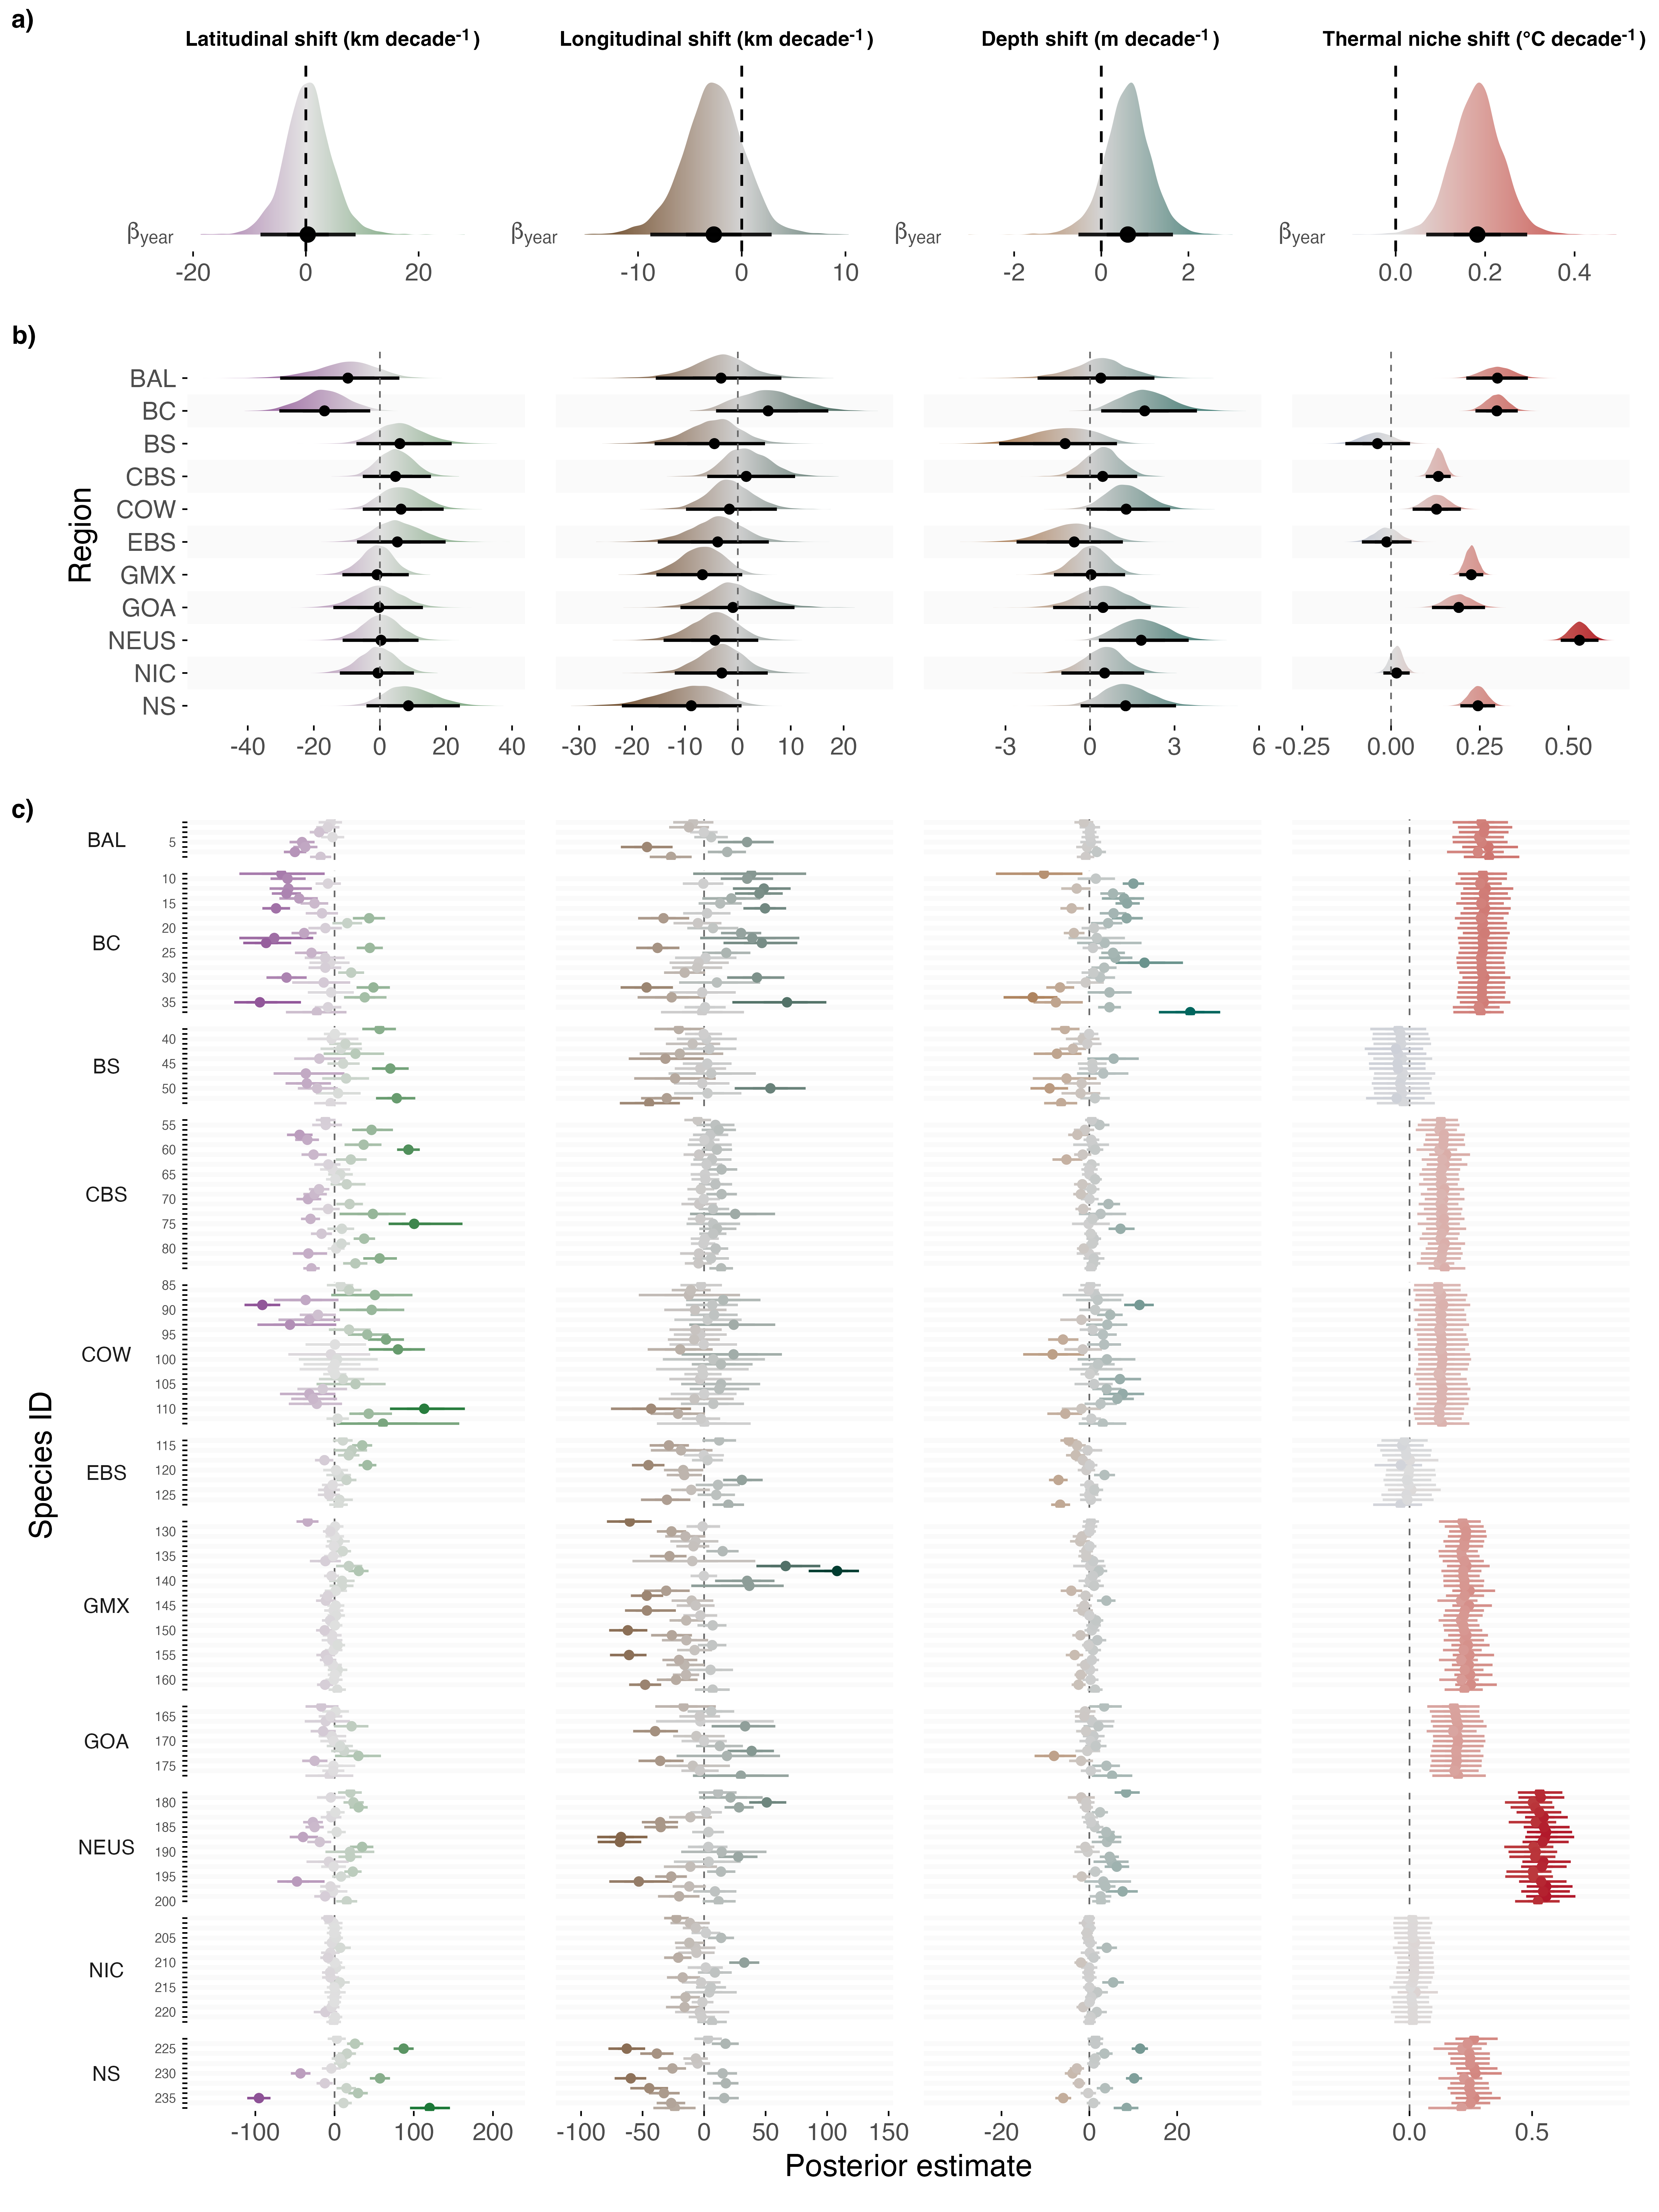
\includegraphics[scale=0.58]{output/figures/slopes.png}
\caption{Trends in distributional shifts of demersal fish species over time, from left to right: latitudinal, longitudinal, depth, and thermal niche shifts. Points and horizontal lines indicate posterior medians and 95\% Bayesian credible intervals.  
(a) Global posterior slopes ($\beta_{year}$),  
(b) Region-specific trends,  
(c) Species-specific trends (rows represent species within regions; see Supplementary XX).  
Density intervals in (a-b) use a continuous gradient reflecting x-values; in (c), color represents median effect size, with more intense colors indicating larger deviations from zero.  
Marine regions: COW = California-Oregon-Washington, NEUS = Northeast U.S. and Scotian Shelf, BS = Barents Sea, NS = North Sea, BC = British Columbia, GOA = Gulf of Alaska, GMX = Gulf of Mexico, NIC = Northern Iberian Coast, EBS = Eastern Bering Sea, CBS = Celtic-Biscay Shelf, BAL = Baltic Sea.}
    \label{fig:effsize}
\end{figure}


\subsection{Species poorly track climate velocities}

Overall, species did not consistently track either the magnitude or the direction of their predicted thermal envelope shifts. Correlations between observed and expected shifts were generally weak, and only about half of the species exhibited alignment in shift direction (Supplementary Table \ref{tab:thermal_envelope}). This pattern was consistent across all regions, with no significant positive correlations observed between expected and actual shifts (Supplementary Table \ref{tab:thermal_envelope_regions}). However, some regions showed higher directional agreement: for example, 79\% of species in the EBS and 69\% in the BS displayed matching latitudinal shift directions between observed and expected values (Supplementary Table \ref{tab:thermal_envelope_regions}).


\begin{table}[ht]
\caption{Correlation and directional agreement between observed shifts and shifts expected by the thermal envelope. The proportion of aligned responses represents the fraction of species for which the expected and observed shifts share the same direction (i.e., sign).}
\centering
\label{tab:thermal_envelope}
\begin{tabular}[t]{l|r|r|r}
\hline
Shift type & $\rho$ & \textit{p}--value & Proportion of aligned responses \\
\hline
Longitudinal & -0.14 & 0.03 & 0.47 \\
\hline
Latitudinal & 0.04 & 0.51 & 0.48 \\
\hline
Depth & -0.01 & 0.85 & 0.53 \\
\hline
\end{tabular}
\end{table}

\subsection{Shift strategies across regions}

Across regions, the first two principal components explained most of the variation in species shifts (67.4–95.5\%), reflecting consistent covariation between spatial redistribution (latitudinal, longitudinal, and depth) and thermal niche shifts. In most regions, PC1 represented a dominant axis along which stronger spatial shifts were associated with weaker thermal niche warming, and vice versa (Fig. \ref{fig:pca}, Fig. \ref{fig:loadings}).

Poleward movement was the spatial axis most negatively correlated with niche warming, especially in regions characterized by broad latitudinal gradients. The strongest correlation occurred in the NS ($\rho = -0.89$), followed by the EBS ($\rho = -0.73$), the NEUS and BS (both $\rho = -0.63$), and then the CBS ($\rho = -0.58$), BC ($\rho = -0.50$), and COW ($\rho = -0.39$).

In regions where poleward movement was less pronounced, other axes became more strongly associated with warming. For instance, longitudinal shifts dominated in the Baltic Sea (BAL, $\rho = -0.80$), while depth shifts played the key role in the GMX ($\rho = -0.70$).
Spatial responses also occurred jointly in certain systems. In the NS, poleward and depth shifts were positively correlated ($\rho = 0.89$). In the NEUS, poleward and eastward shifts tended to co-occur ($\rho = 0.82$), while in the BAL, eastward and depthward shifts were correlated ($\rho = 0.62$).
In contrast, correlations with warming were minimal in the NIC and the GOA, and no clear relationship emerged.

\begin{figure}[h]
    \centering
        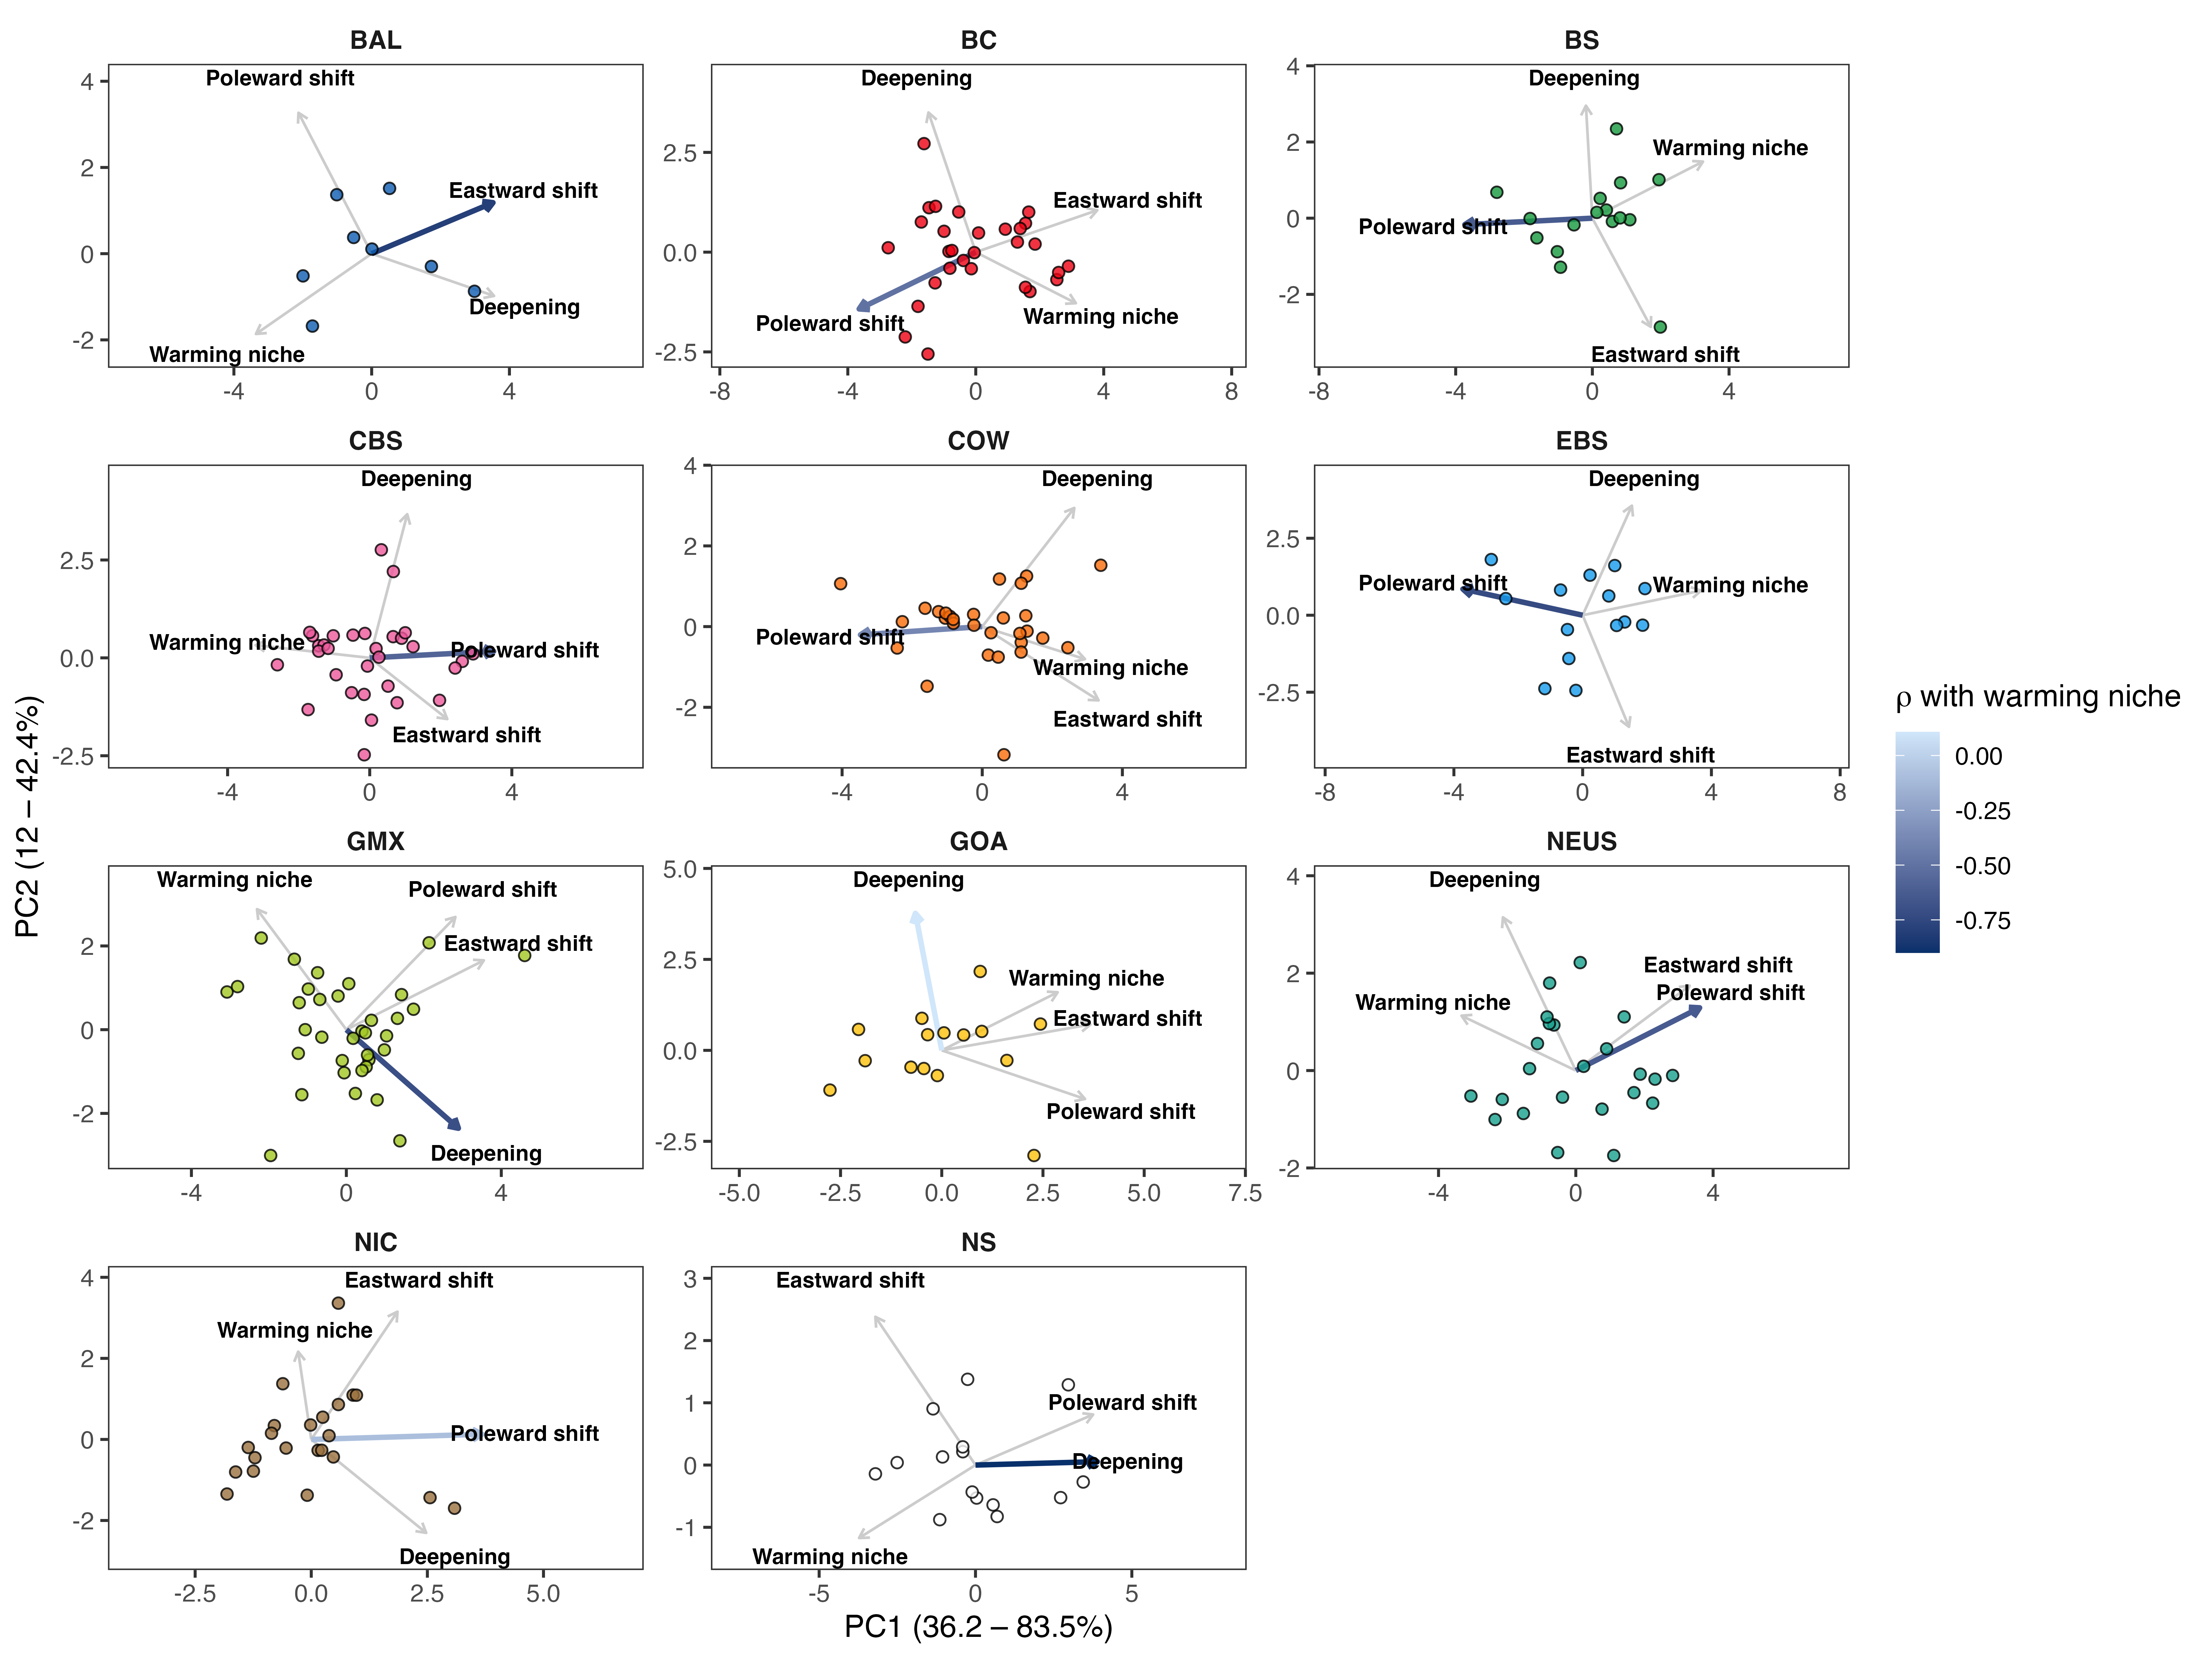
\includegraphics[scale=0.6]{output/figures/pca.png}
    \caption{Principal component analysis (PCA) of species shifts by region. Each panel shows species scores (points) and shift loadings (arrows). Blue arrows highlight the dominant shift strategy used to avoid niche warming in each region, with color intensity indicating the strength of its correlation ($\rho$) with thermal niche warming (darker blue = stronger negative correlation). The percentages shown on the PC1 and PC2 axis labels represent the range of variance explained across regions. Regions are represented by the following codes:
COW = California-Oregon-Washington states, NEUS = Northeast U.S. and Scotian Shelf, BS = Barents Sea, NS = North Sea, BC = British Columbia, GOA = Gulf of Alaska, GMX = Gulf of Mexico, NIC = Northern Iberian Coast, EBS = Eastern Bering Sea,
CBS = Celtic-Biscay Shelf,
BAL = Baltic Sea.
}
    \label{fig:pca}
\end{figure}

\subsection{Limited evidence for shift strategies predicting abundance trajectories}

Across regions, relationships between abundance trends and distributional shifts were generally weak (Fig. \ref{fig:win_lose}a). However, a significant effect of latitudinal shifts was detected, indicating that species moving poleward more rapidly tended to experience stronger declines in abundance (slope = –0.003, $R^2$ = 0.02, $p$ = 0.034). No significant associations were found for longitudinal (slope = 0.001, $R^2$ = 0, $p$ = 0.45), depth (slope = 0.001, $R^2$ = 0, $p$ = 0.91), or thermal niche shifts (slope = -0.009, $R^2$ = 0, $p$ = 0.98).

The relationships also varied markedly across regions with no single shift dimension consistently related to changes in abundance (Fig. \ref{fig:win_lose}b). However, in the NEUS, abundance declined with poleward- (slope = –0.018, $p$ = 0.011, $R^2$ = 0.27), eastward- (slope = –0.010, $p$ = 0.050, $R^2$ = 0.17), and PC1 shifts (slope = –0.265, $p < 0.001$, $R^2$ = 0.31), with PC1 representing a composite of poleward and eastward movement opposed to thermal niche warming (Supplementary Fig. \ref{fig:loadings}). In contrast, species expanding into deeper habitats tended to increase in abundance (slope = 0.137, $p$ = 0.011, $R^2$ = 0.27).

In the BAL, poleward shifts were strongly associated with abundance declines (slope = –0.034, $p$ = 0.025, $R^2$ = 0.60). Deeper niche use tended to correspond with higher abundance (slope = 0.555, $p$ = 0.089, $R^2$ = 0.41), and PC1, reflecting stronger eastward and depth shifts coupled with reduced poleward and thermal niche shifts— was positively related to abundance (slope = 0.200, $p$ = 0.012, $R^2$ = 0.19; Supplementary Fig. \ref{fig:loadings}). In the NIC, abundance declined with PC1 (slope = –0.175, $p < 0.001$, $R^2$ = 0.16), which primarily captures broad spatial displacement, including poleward, eastward, and depth shifts. In the GOA, abundance declined with both eastward shifts (slope = –0.016, $p$ = 0.052, $R^2$ = 0.26) and PC1 (slope = –0.138, $p$ = 0.021, $R^2$ = 0.09), the latter reflecting combined poleward/eastward movement and thermal niche warming. No other regions showed significant associations between abundance trends and spatial or niche shifts.


\begin{figure}[h]
    \centering
    \includegraphics[scale=0.5]{output/figures/win_lose.png}
    \caption{
 Relationships between species abundance trends and distributional shifts. (a) Global slopes across all regions for each shift dimension (poleward, eastward, depth, and thermal niche). Reported in the top right are the estimated slope, $R^2$, and $p$-values. (b) Region-specific coefficients, illustrating how the strength and direction of associations vary among systems. Points and lines indicate means and 95\% confidence intervals. Negative values denote declining abundance with increasing shift magnitude, while positive values indicate increasing abundance. Region codes: COW = California–Oregon–Washington, NEUS = Northeast U.S. and Scotian Shelf, BS = Barents Sea, NS = North Sea, BC = British Columbia, GOA = Gulf of Alaska, GMX = Gulf of Mexico, NIC = Northern Iberian Coast, EBS = Eastern Bering Sea, CBS = Celtic–Biscay Shelf, BAL = Baltic Sea.}
    \label{fig:win_lose}
\end{figure}


\section{Discussion}

Marine biodiversity is undergoing rapid reorganization under ocean warming, with many studies reporting net poleward and deepward shifts as species track their thermal niches \citep{parmesan_globally_2003, perry_climate_2005, dulvy_climate_2008}. Yet these latitudinal and vertical redistributions represent only a subset of possible responses, and they are typically examined independently \citep{fredston_reimagining_2025}. This unidimensional perspective limits our ability to understand how species respond across the full range of ecological pathways available to them, and whether such movements reduce their exposure to warming. To address this gap, we developed a multidimensional framework that jointly quantifies horizontal, vertical, and thermal niche dynamics for more than 200 fish populations across 11 rapidly warming continental shelf regions. We show that redistribution is more variable, less coherent, and less effective at buffering populations from ocean warming than previously assumed. Moreover, associations between redistribution strategies and abundance trends were weak, indicating that movement alone is not a reliable predictor of population resilience under climate change.

Across regions, we found little evidence for net poleward migration. Instead, horizontal shifts tended to balance out, with some species or regions showing northward movement while others shifted southward or remained stationary. This lack of a consistent cross-regional signal contrasts with global syntheses that emphasize widespread poleward redistribution, and highlights the importance of accounting for regional variability in climate trajectories, habitat geometry, and species’ ecological constraints. The absence of a dominant poleward fingerprint suggests that latitudinal movement alone is not a universal pathway of thermal niche tracking.


%Using a multidimensional framework applied to two to three decades of standardized bottom-trawl surveys, we tracked horizontal, vertical, and thermal niche dynamics of demersal fish populations across 11 rapidly warming continental shelf regions. We show that despite substantial warming there are overall weak net cross-regional patterns in range shift, with no strong or consistent signal of poleward movement. 
%Many species did not track their thermal niches through spatial redistribution. Instead, their movements have been poorly aligned with regional warming, leaving populations in environments that have warmed in step with local ocean trends. These patterns indicate that simple assumptions—such as species universally moving poleward, deeper, or into cooler habitats—are inadequate. Rather, the redistribution of marine biodiversity is shaped by a complex interplay of processes, including ecological constraints, limited dispersal, habitat fragmentation, and non-thermal factors such as oxygen availability, prey dynamics, and biotic interactions \citep{sunday_species_2015,dulvy_climate_2008,deutsch_climate_2015,siren_interactive_2020}.

% Our findings differ from global syntheses that report consistent poleward or deepening shifts in marine species \citep[e.g.,][]{poloczanska_global_2013, burrows_geographical_2014}. Several differences in data and methods, rather than species’ actual responses, may explain this difference. First, global syntheses often rely on literature-reported shifts, which can bias results toward species where changes are expected or easiest to detect. Second, most meta-analyses do not propagate uncertainty from the original estimates \citep{rubenstein_climate_2023}, which makes it hard to know how reliable the reported trends are. Third, analytical choices strongly influence estimated shift rates. For example, estimates based on presence–absence data often differ from those based on abundance data, and using range edges instead of distribution centroids can also change results. These differences can sometimes be larger than the effects of the underlying ecological drivers \citep{brown_2016}. Finally, some long-term range-shift studies overlook changes in survey design and effort over time. Sites may be added or removed, and sampling intensity can increase or decrease across years or regions. Ignoring these changes can hide real trends or create false ones \citep{thorson_model-based_2016}.

% say how we overcome this

% By drawing on standardized, fishery-independent bottom-trawl surveys with consistent sampling designs across regions, our study minimizes these methodological artifacts. This provides a clearer signal of true biological responses to ocean warming and likely explains why we detect weaker and more variable cross-regional patterns compared to studies synthesizing heterogeneous data sources.

%One can expect that species shifting their ranges quickly are the ones better coping with climate change, maintaining stable or growing populations as they track their preferred thermal habitats. Our results challenge this view. Across regions, relationships between range shifts and abundance trends were generally weak, indicating that movement alone is not a reliable predictor of demographic success. At a cross-regional scale, we found that species moving poleward more rapidly tended to experience stronger declines in abundance. This finding is consistent with recent work by \citet{chiaikin_2024}, who also reported negative associations between poleward shifts and population trends.

%One possible explanation is a detection artifact: species moving beyond the boundaries of survey domains may appear to decline, even if their total population size remains stable or increases. This may be occurring in the NEUS–SS region, where north-eastward shifts were associated with declines, while populations shifting deeper—yet remaining within the survey area—showed increases. Alternatively, negative associations may reflect real demographic costs of displacement, such as moving into suboptimal habitats or encountering greater competition and predation in newly occupied areas \citep{pinsky_marine_2013, fredston_reimagining_2025}. 
%Regardless of this, this might be a problem for fisherman as stock shifitng north might means less accessiability and higher fuel coasts.
%Regional contrasts highlight that there is no single “safe” response to climate change. In the Baltic, poleward shifts corresponded with declines, whereas depth and eastward shifts supported abundance. In NIC and GOA, broad spatial displacement along multiple axes was associated with negative population trends. These divergent patterns suggest that the relationship between redistribution and demographic outcomes is highly context dependent, shaped by local oceanography, habitat availability, and species-specific life histories \citep{dulvy_climate_2008, sunday_species_2015, deutsch_climate_2015}. Together, our findings caution against assuming that poleward movement universally signals resilience to warming. Instead, tracking abundance alongside redistribution is essential for identifying species at greatest risk under accelerating climate change. Improved understanding of species redistribution requires expansion of monitoring programs
% also the opposite is true so that more thermal niche warming doesn't mean spescie are losing ..

% something like region-wise shifts behave as expected. e.g. BC Columbia steep depth gradient, North Sea going North means also going deep, etc. etc.

% in the winner loser part mention that species shifting north faster might be declining because they escape the survey domain 

% estimate of range shifts are in the same ballpark as 

% weak agreement with thermal envelopes. Our comparison of observed and expected thermal envelope shifts revealed poor tracking of both the magnitude and direction of climate velocities. Only about half of species exhibited shifts in the expected direction, and correlations between observed and predicted rates were weak. This mismatch is consistent with previous work \citep{gordo-vilaseca_over_2023} and suggest influences of other factors, wether restricted geographies preventing shifts, biological interactions orstocasticty or recovery from perturbations..In contrast to overall weak net effects.. Some regions geographical and oceanic feature prevented shift... such as

\section{Acknowledgements}

\section{Author contributions}

\section{Data Availability Statement}

\section{Funding}
BUSEFUL
Max grant?
Dani? Eric? Sean? 

\end{spacing}

%\bibliographystyle{fishfish}
\bibliography{references}

\clearpage

\renewcommand{\thefigure}{S\arabic{figure}}
\renewcommand{\thetable}{S\arabic{table}}
\setcounter{figure}{0}
\setcounter{table}{0}
\addtocontents{toc}{\protect\setcounter{tocdepth}{0}}
\onehalfspacing
\linenumbers
\resetlinenumber
\setcounter{secnumdepth}{0}
\setcounter{page}{1}
\setcounter{equation}{0}
\nolinenumbers
\floatplacement{table}{H}
\floatplacement{figure}{H}

\section{Supplementary Information}

\begin{table}

\caption{Model comparison based on leave-one-out cross-validation (LOO).  MVN denotes a multivariate normal distribution, while Student-t $+$ MVN specifies a univariate Student-t distribution for each response combined with multivariate normal random effects.
  The expected log predictive density (ELPD) reflects out-of-sample predictive accuracy, with higher values indicating better performance. ELPD differences are shown relative to the best-fitting model, so negative values indicate worse fit. The standard error (SE) of the difference reflects uncertainty; differences large relative to SE suggest meaningful performance gaps.}
\centering
\begin{tabular}[t]{lrr}
\toprule
Model & ELPD difference & SE difference\\
\midrule
<<<<<<< HEAD
Student-t \$+\$ MVN & 0.0 & 0.00\\
=======
Student-t $+$ MVN & 0.0 & 0.00\\
>>>>>>> f3da522 (first table)
MVN & -169139.8 & 11054.05\\
\bottomrule
\end{tabular}
\end{table}


\newpage

\begin{figure}[h]
    \centering
        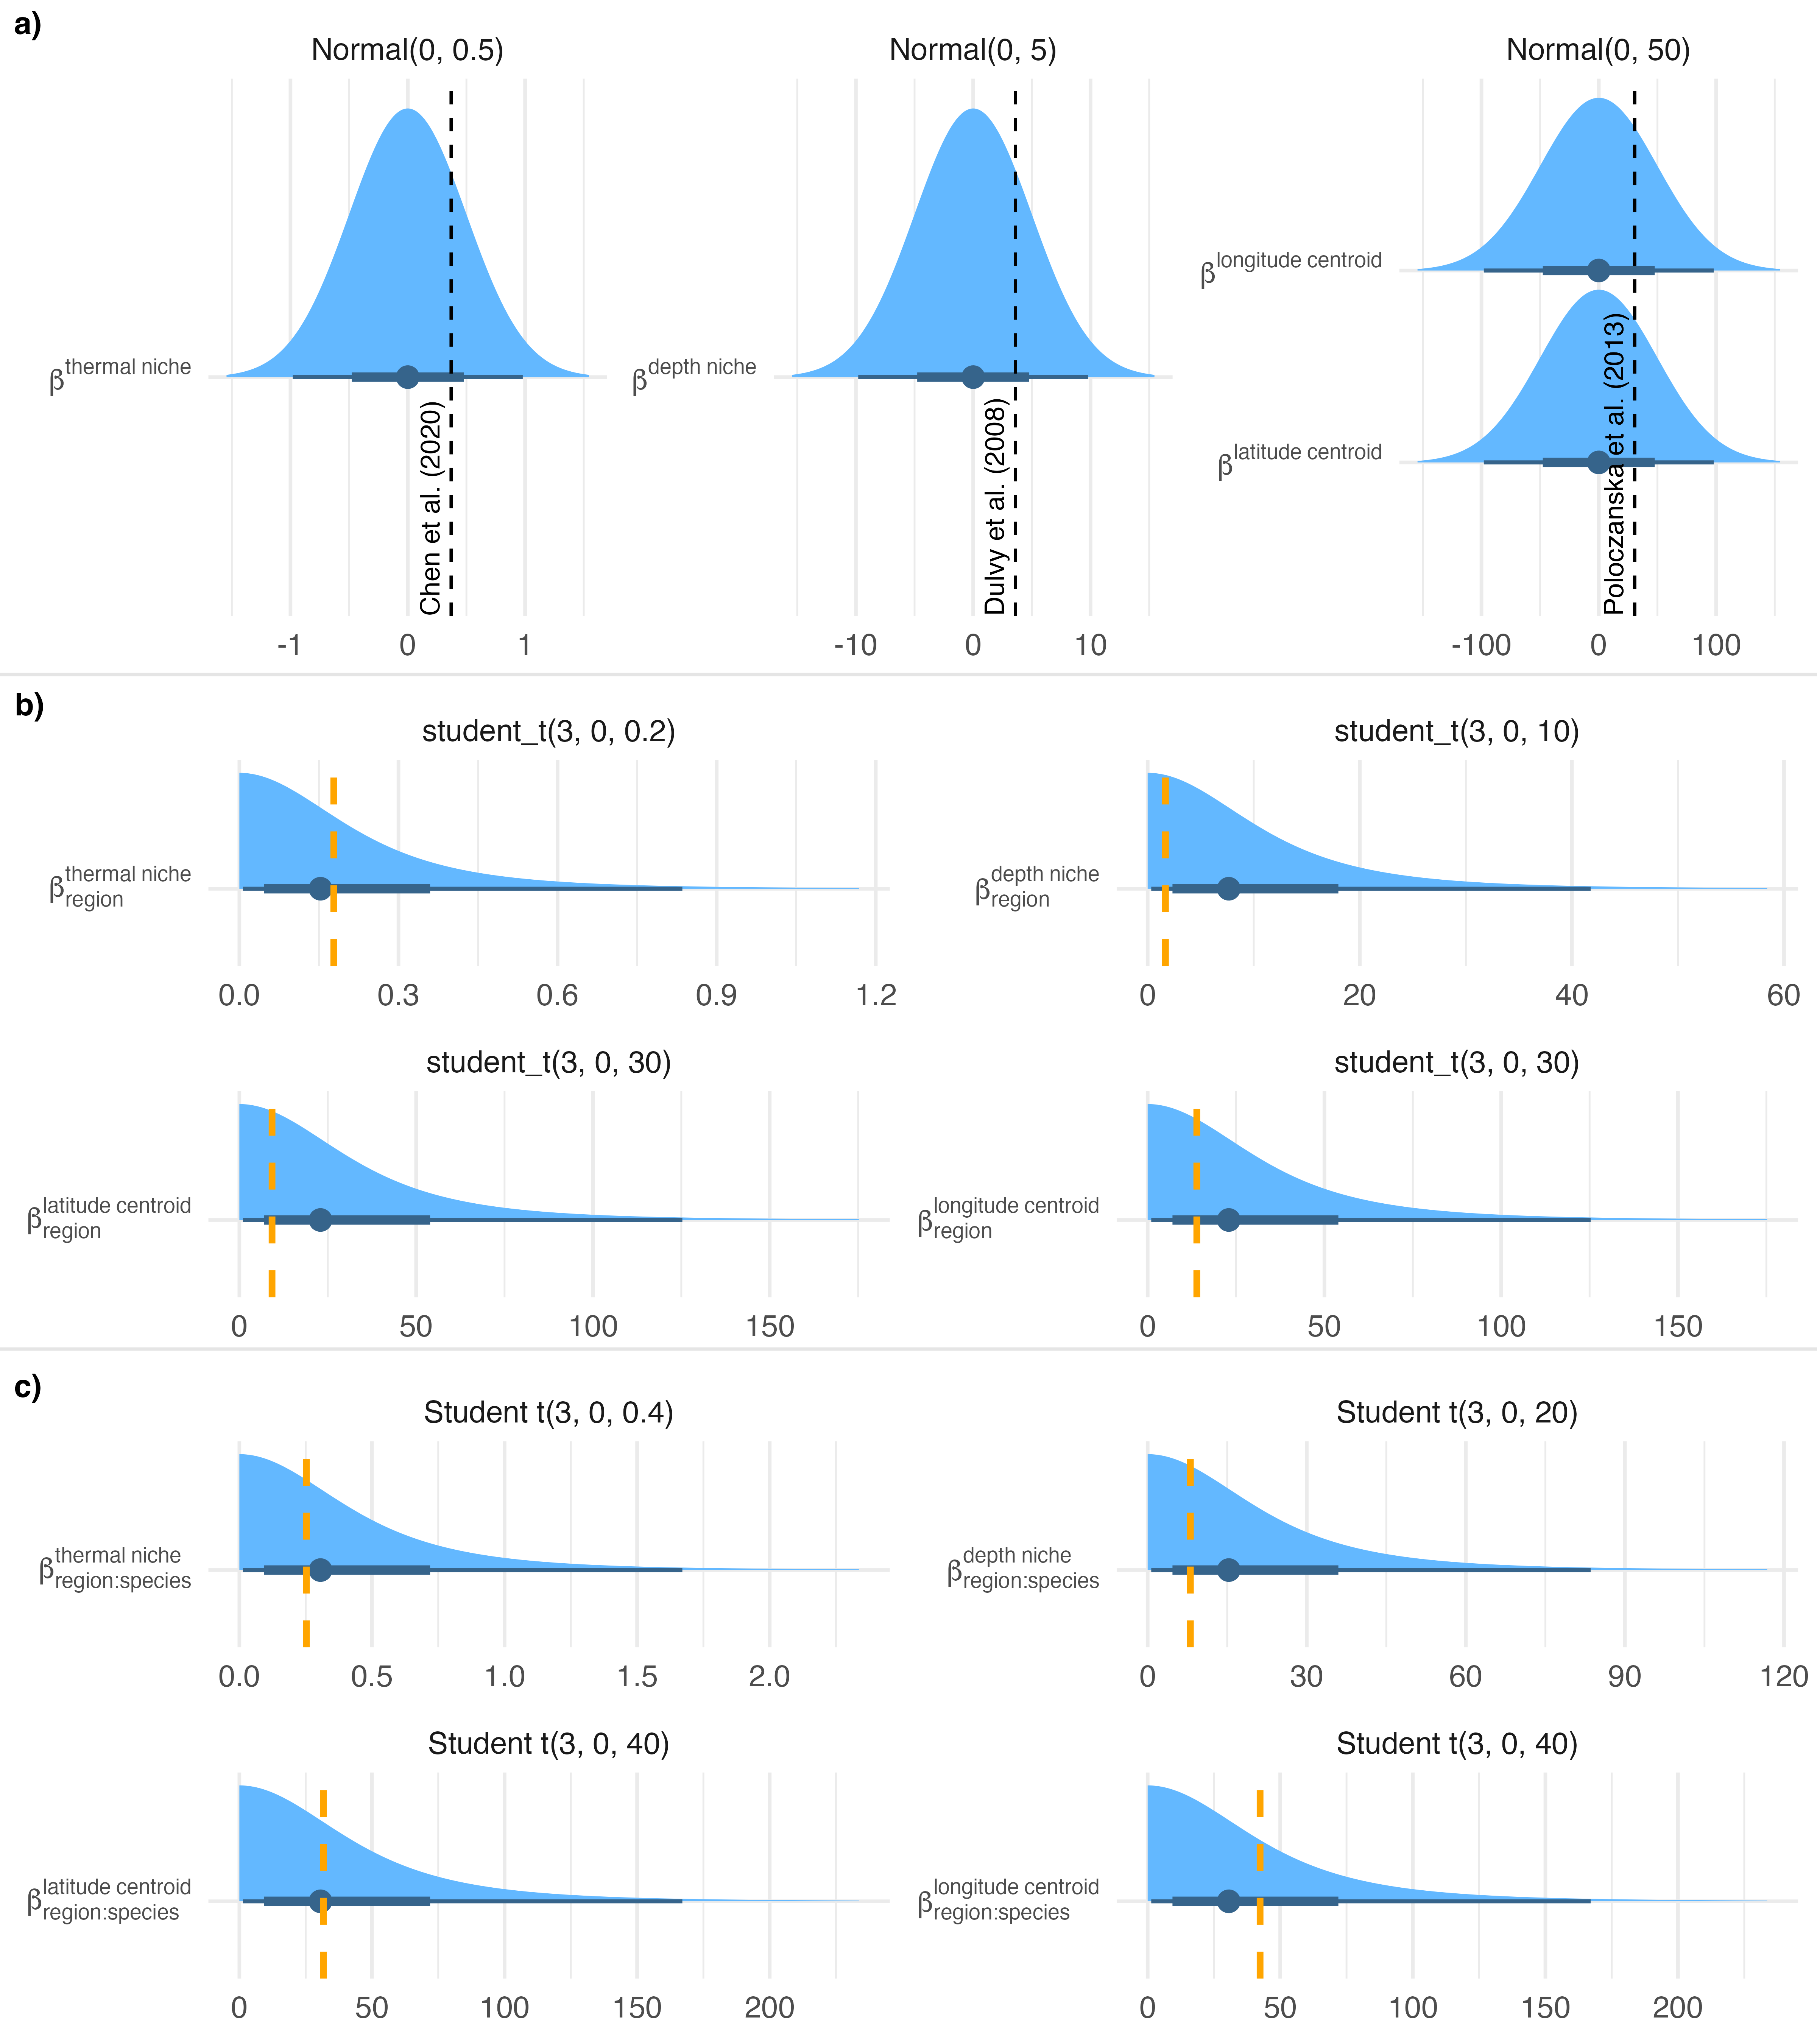
\includegraphics[scale=0.7]{output/figures/prior_checks.png}
    \caption{(a) Prior distributions plotted against literature-reported values (black dashed line), showing that reported estimates fall within the prior ranges.
 Region-level (b) and species-within-region (c) standard deviations (SD) of the year slope estimates. Orange dashed lines indicate empirical SD estimates, showing that observed variability is compatible with the specified prior ranges.
}
    \label{fig:priors}
\end{figure}

\newpage

\begin{figure}[h]
    \centering
        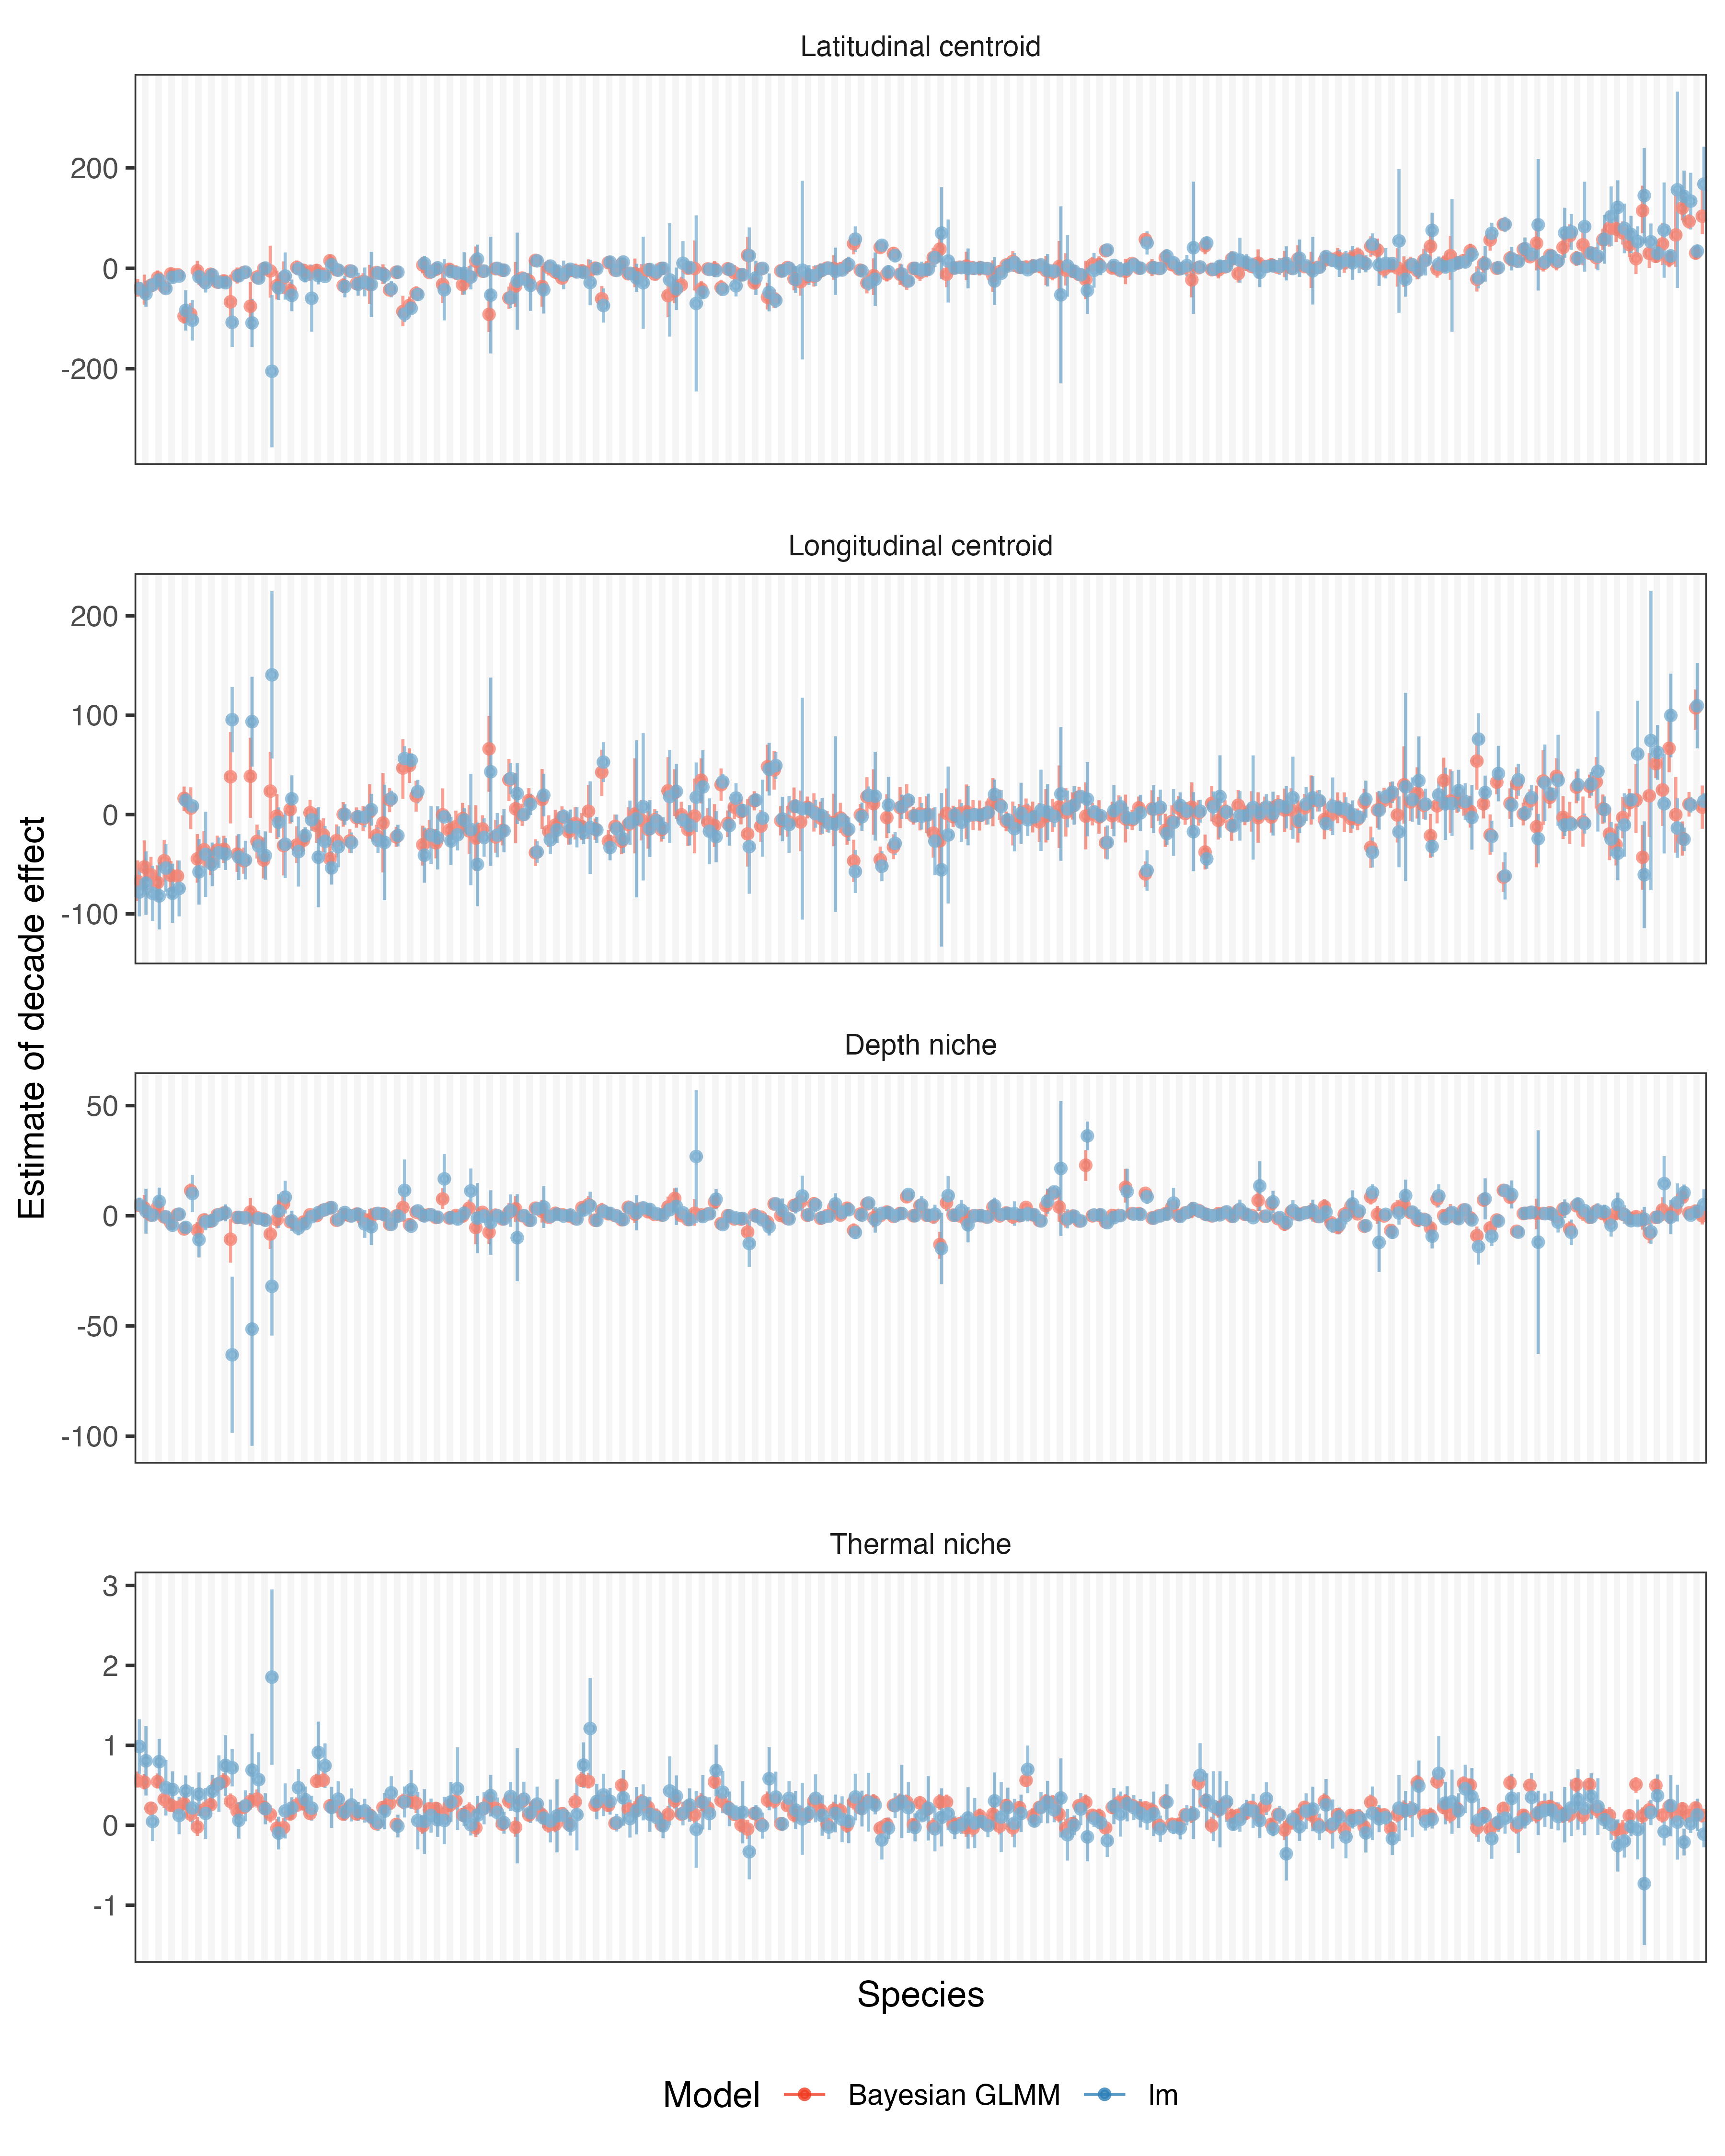
\includegraphics[scale=0.7]{images/shrinkage_slopes.png}
    \caption{Comparison of estimated decade effects from our Bayesian mixed-effects model (red) versus separate single-species models (blue) for each species. The hierarchical model applies shrinkage, pulling extreme species-level slopes toward the region mean and the grand mean based on the collective evidence across region and species.
}
    \label{fig:shrinkage}
\end{figure}

\newpage

\begin{figure}[h]
    \centering
    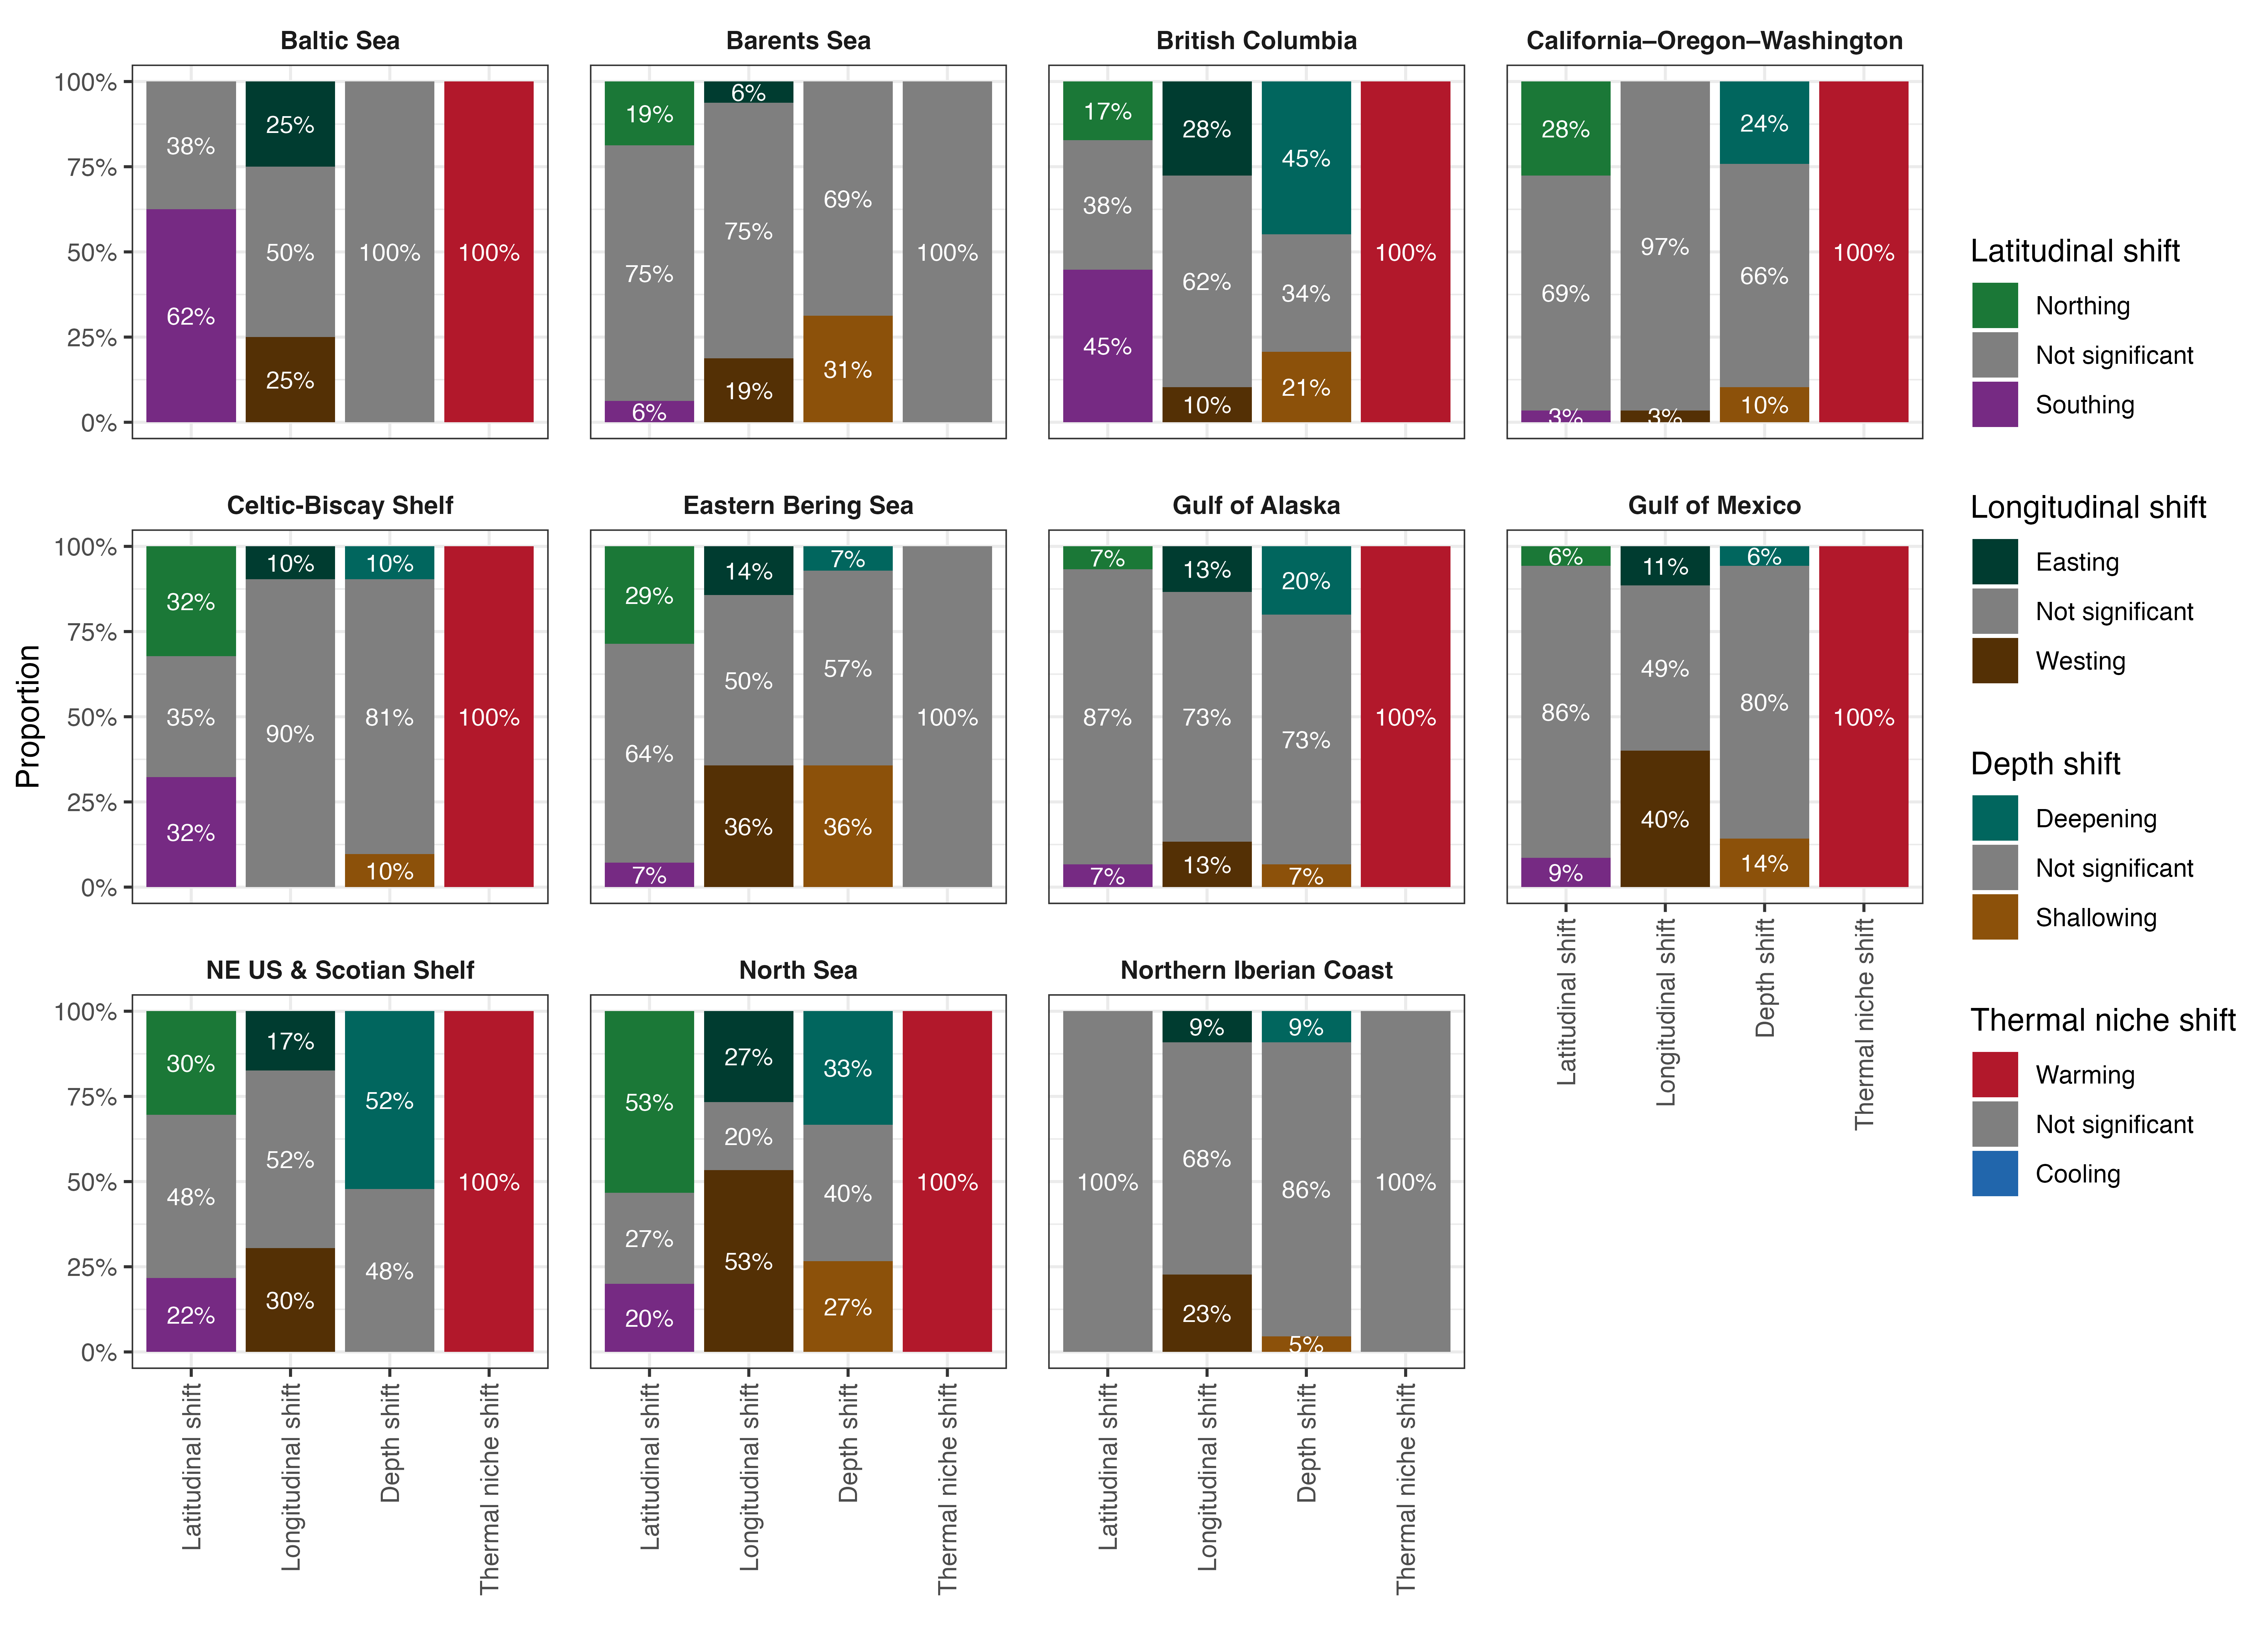
\includegraphics[scale=.65]{output/figures/prop_sign.png}
    \caption{Proportion of significant species-level responses across regions and shift types, where significance is defined as the 95\% Bayesian credible interval of the species-specific slope excluding zero. 
Bars show the percentage of species with significant latitudinal (northing/southing), longitudinal (easting/westing), depth (deepening/shallowing), and thermal niche (warming/cooling) shifts. 
Each bar is divided by direction of change, and numbers within the bars indicate the proportion of species in each category. 
Grey segments denote non-significant responses.}
    \label{fig:prop_sign}
\end{figure}


\newpage

\begin{table}[ht]
\caption{Correlation and directional agreement between observed shifts and shifts expected by the thermal envelope across regions. 
The proportion of aligned responses represents the fraction of species for which the expected and observed shifts share the same direction (i.e., sign). 
$\rho$ denotes the Pearson correlation coefficient between observed and expected shifts. 
Region codes: COW = California–Oregon–Washington, NEUS = Northeast U.S. and Scotian Shelf, BS = Barents Sea, NS = North Sea, BC = British Columbia, GOA = Gulf of Alaska, GMX = Gulf of Mexico, NIC = Northern Iberian Coast, EBS = Eastern Bering Sea, CBS = Celtic–Biscay Shelf, BAL = Baltic Sea.}
\centering
\label{tab:thermal_envelope_regions}
\begin{tabular}{l l r r r}
\hline
Region & Type of shift & Proportion aligned & $\rho$ & \textit{p}--value \\
\hline
BAL & Longitudinal shift & 0.38 & -0.55 & 0.16 \\
BAL & Latitudinal shift  & 0.62 & 0.32  & 0.44 \\
BAL & Depth shift        & 0.38 & -0.15 & 0.72 \\
BC  & Longitudinal shift & 0.34 & 0.16  & 0.40 \\
BC  & Latitudinal shift  & 0.31 & 0.00  & 0.99 \\
BC  & Depth shift        & 0.59 & -0.08 & 0.68 \\
BS  & Longitudinal shift & 0.38 & -0.46 & 0.07 \\
BS  & Latitudinal shift  & 0.69 & 0.50  & 0.05 \\
BS  & Depth shift        & 0.56 & 0.06  & 0.83 \\
CBS & Longitudinal shift & 0.61 & 0.09  & 0.61 \\
CBS & Latitudinal shift  & 0.32 & -0.30 & 0.10 \\
CBS & Depth shift        & 0.52 & -0.05 & 0.78 \\
COW & Longitudinal shift & 0.38 & -0.15 & 0.47 \\
COW & Latitudinal shift  & 0.54 & 0.07  & 0.75 \\
COW & Depth shift        & 0.58 & 0.06  & 0.76 \\
EBS & Longitudinal shift & 0.36 & -0.31 & 0.29 \\
EBS & Latitudinal shift  & 0.79 & 0.25  & 0.39 \\
EBS & Depth shift        & 0.57 & 0.01  & 0.97 \\
GMX & Longitudinal shift & 0.54 & -0.11 & 0.54 \\
GMX & Latitudinal shift  & 0.46 & -0.13 & 0.44 \\
GMX & Depth shift        & 0.49 & 0.26  & 0.13 \\
GOA & Longitudinal shift & 0.47 & 0.06  & 0.83 \\
GOA & Latitudinal shift  & 0.53 & -0.11 & 0.70 \\
GOA & Depth shift        & 0.60 & -0.19 & 0.49 \\
NEUS & Longitudinal shift & 0.43 & -0.01 & 0.96 \\
NEUS & Latitudinal shift  & 0.48 & -0.11 & 0.62 \\
NEUS & Depth shift        & 0.65 & 0.19  & 0.38 \\
NIC  & Longitudinal shift & 0.55 & -0.04 & 0.88 \\
NIC  & Latitudinal shift  & 0.41 & 0.30  & 0.17 \\
NIC  & Depth shift        & 0.32 & -0.43 & 0.04 \\
NS   & Longitudinal shift & 0.53 & -0.24 & 0.38 \\
NS   & Latitudinal shift  & 0.53 & 0.12  & 0.67 \\
NS   & Depth shift        & 0.60 & 0.16  & 0.56 \\
\hline
\end{tabular}
\end{table}

\newpage
\begin{figure}[h]
    \centering
        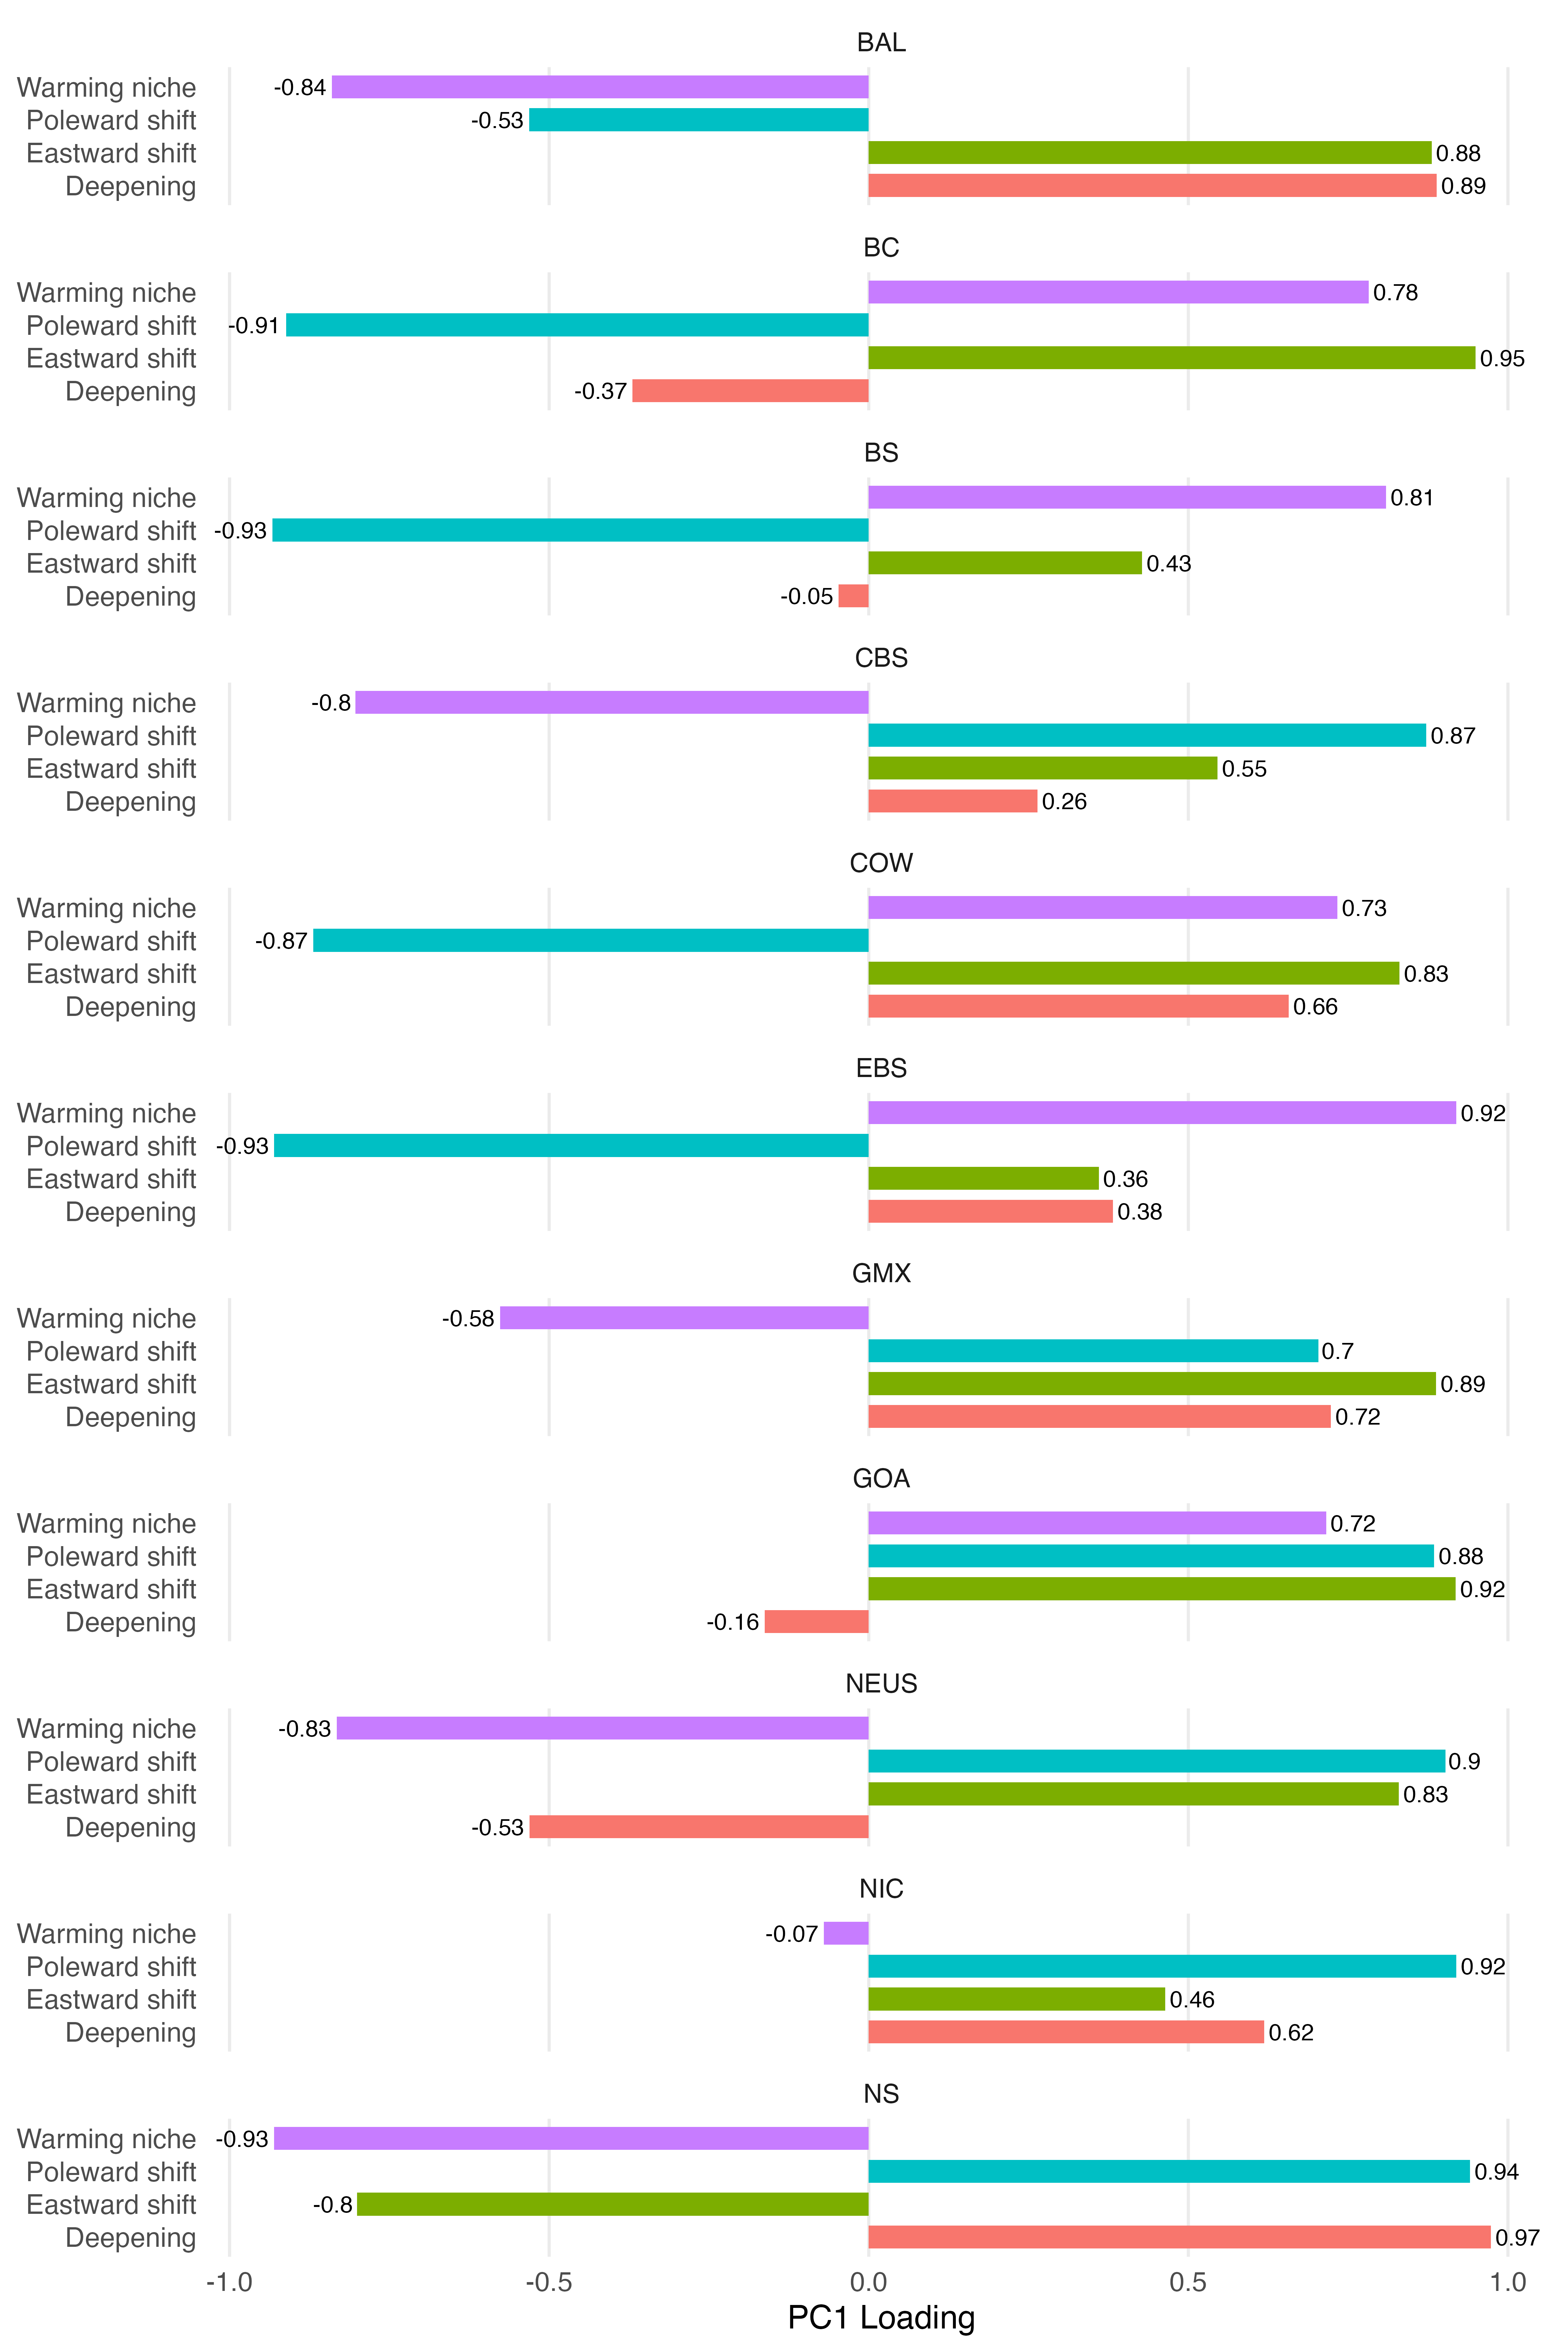
\includegraphics[scale=0.6]{output/figures/loadings.png}
    \caption{PC1 loadings for each region. Bars represent the magnitude and direction of the loading for each outcome, with values on the side of the bars. Positive values indicate a positive association with PC1, while negative values indicate a negative association.
}
    \label{fig:loadings}
\end{figure}

\clearpage

\subsubsection{References}
\begin{hangparas}{1em}{1}
Chen, Z., Kwon, Y.-O., Chen, K., Fratantoni, P., Gawarkiewicz, G. \& Joyce, T.M. (2020)
Long‐Term SST Variability on the Northwest Atlantic Continental Shelf and Slope. Geophysical Research Letters 47(1), e2019GL085455.
URL \url{https://agupubs.onlinelibrary.wiley.com/doi/10.1029/2019GL085455}. Publisher: AGU.

Dulvy, N.K., Rogers, S.I., Jennings, S., Stelzenmüller, V., Dye, S.R. \& Skjoldal, H.R. (2008)
Climate change and deepening of the North Sea fish assemblage: a biotic indicator of warming seas. Journal of Applied Ecology 45(4), 1029–1039.
URL \url{https://onlinelibrary.wiley.com/doi/10.1111/j.1365-2664.2008.01488.x}. Publisher: British Ecological Society.

Poloczanska, E.S., Brown, C.J., Sydeman, W.J., Kiessling, W. et al. (2013)
Global imprint of climate change on marine life. Nature Climate Change 3(10), 919–925.
URL \url{https://www.nature.com/articles/nclimate1958}. Publisher: Nature Publishing Group.

\end{hangparas}

\end{document}